\documentclass[11pt,letterpaper,titlepage]{article}
\usepackage{fancyhdr}
\usepackage[left=0.75in, right=0.75in, bottom=1.0in]{geometry}
\usepackage{lastpage}
\usepackage{titleref}
\usepackage{booktabs}
\usepackage{appendix}
\appendixtitleon
\appendixtitletocon

\makeatletter

%================== List of figures and tables mods
\usepackage{tocloft}
\usepackage[labelfont=bf]{caption}

\renewcommand{\cftfigpresnum}{Figure\ }
\renewcommand{\cfttabpresnum}{Table\ }

\newlength{\mylenf}
\settowidth{\mylenf}{\cftfigpresnum}
\setlength{\cftfignumwidth}{\dimexpr\mylenf+1.5em}
\setlength{\cfttabnumwidth}{\dimexpr\mylenf+1.5em}



\newcommand{\half}{\frac{1}{2}}


%=================== Graphics
\usepackage{graphicx}
\usepackage[breakwords]{truncate}
\usepackage{float}
\usepackage{array}
\usepackage{amsmath}
\usepackage{mdframed}
\usepackage{fancyvrb}
\usepackage{float}
\usepackage{cancel}
\usepackage{amssymb}
\graphicspath{ {images/} }
\usepackage[usenames,dvipsnames,svgnames,table]{xcolor}
\usepackage[defaultlines=2,all]{nowidow}
\usepackage{listings}
\usepackage{color}
\definecolor{Brown}{cmyk}{0,0.81,1,0.60}
\definecolor{OliveGreen}{cmyk}{0.64,0,0.95,0.40}
\definecolor{CadetBlue}{cmyk}{0.62,0.57,0.23,0}
\usepackage{pdflscape}
\usepackage{relsize}
\usepackage{verbatim}
\usepackage{tabto}


%=================== Settings
\renewcommand{\baselinestretch}{1.2}
\definecolor{gray}{rgb}{0.4 0.4 0.4}
\newcommand{\stimes}{{\times}}
\setcounter{MaxMatrixCols}{20}

\begin{document}
\newcommand{\NSCDOCNUMBR}{NSC-REP-15-X}         %Put document number here
\newcommand{\NSCDOCSUBJT}{TECHNICAL REPORT: }   %Put document subject here
\newcommand{\NSCDOCTITLE}{$THERMOALPHA$ - Two-phase System level Thermal-Hydraulics in $ChiTech$}       %Put document title here
\newcommand{\NSCDOCDATE} {May, 2017}    %Put document date here
\newcommand{\NSCDOCREV}  {Rev 1.0} %Put revision number here

\lstset{language=C++,frame=ltrb,framesep=4pt,basicstyle=\linespread{0.8} \small,
	keywordstyle=\ttfamily\color{OliveGreen},
	identifierstyle=\ttfamily\color{CadetBlue}\bfseries,
	commentstyle=\color{Brown},
	stringstyle=\ttfamily,
	showstringspaces=ture }


%################################# TITLE PAGE ########################
\begin{titlepage}
	\pagestyle{fancy}
	\vspace*{1.0cm}
	\centering
	%\includegraphics{NSC_Logo} \par
	\vspace{1cm}
	%\centering
	%{\Large\bfseries  \NSCDOCNUMBR   \par}
	\vspace{.25cm}
	%\centering
	{\Large\bfseries  \NSCDOCSUBJT \par} 
	{\Large\bfseries \NSCDOCTITLE  \par}
	\vspace{1cm}
	{\Large \NSCDOCDATE \par}
	\vspace{1.0cm}
	{\Large Jan Vermaak \par}
	{\Large \NSCDOCREV \par}
		
	\begin{comment}
	\renewcommand{\arraystretch}{2.0}
	\begin{tabular}{| m{2.5cm} | m{4.5cm} | m{4.5cm} |}
		\cline{2-3}
		\multicolumn{1}{c|}{} & \bfseries{Name} & \bfseries{Signature \& Date} \\ \hline
		\bfseries{Prepared} &     &     \\ \hline
		\bfseries{Reviewed} &     &     \\ \hline
		\bfseries{Reviewed} &     &     \\ \hline
	    \bfseries{Approved} &     &     \\ \hline
	\end{tabular} \par
	\end{comment}
	\begin{center}
		\begin{minipage}[c]{0.45\textwidth}
			\begin{figure}[H]
			
				
\includegraphics[width=3in]{Logo2_Medium.png}
			\end{figure}
		\end{minipage}
	\end{center}
	\vspace{2cm}
	%NSC-FRM-15-1 Rev.1
\end{titlepage}


\pagestyle{fancy}
\rfoot{Page \thepage \ of \pageref{LastPage}}
%\cfoot{NSC-FRM-15-1 Rev.1}
\cfoot{}
\lfoot{\truncate{14cm}{\NSCDOCTITLE}}
\rhead{}
\chead{\currentname}
\lhead{}
\renewcommand{\footrulewidth}{0.4pt}
\tableofcontents
\addtocontents{toc}{~\hfill\textbf{Page}\par}

\listoffigures
%\listoftables
\chead{Contents}


\newpage
\chead{1 Conservation equations}
\section{Conservation equations}
The overall objective of simulating system level thermal-hydraulics is to solve the following four field variables \textbf{for each phase}:
\begin{itemize}
\item Pressure, $P$
\item Internal energy, $u$
\item Velocity, $v$
\item Density, $\rho$
\end{itemize}

\vspace{0.25cm}
\noindent
In order to do this we apply the conservation equations to the control volume shown in Figure \ref{figure:ZZZ_ControlVolume} below. In this configuration the conservation of momentum is calculated over the connection of adjoining control volumes in \textbf{staggered grid} fashion. This choice is convenient because it allows control volumes to be conveniently connected through pressure as well to allow for pressure loss devices to be incorporated at junctions instead of inside control volumes.
	\begin{center}
		\begin{minipage}[c]{0.85\textwidth}
	
			\begin{figure}[H]
			
				%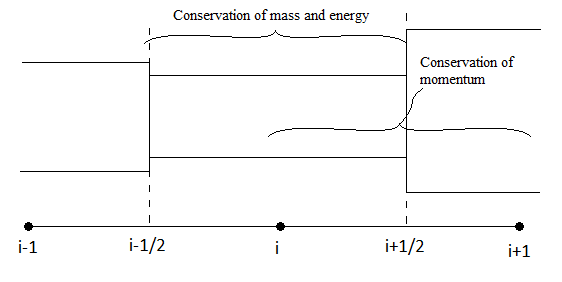
\includegraphics[width=562px]{ZZZ_ControlVolume.png}
				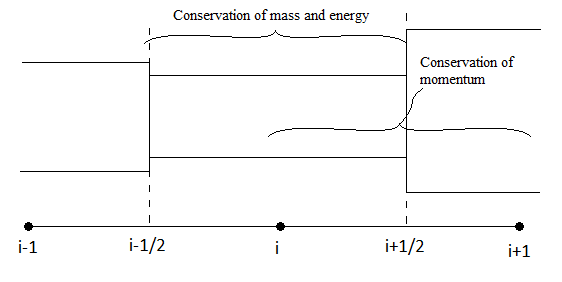
\includegraphics{ZZZ_ControlVolume.png}
				\caption{Simple layout of control volumes.}
				\label{figure:ZZZ_ControlVolume}
			\end{figure}
		\end{minipage}
	\end{center}
\vspace{0.5cm}

\newpage
\subsection{Conservation of Mass}
The conservation of mass requires as a function of time, $t$, that the total mass of the system, $\alpha_g \rho_g+\alpha_f\rho_f$, be equal to that streaming in minus that streaming out \textbf{(subscript $g$ denotes steam and $f$ denotes liquid)}:

\begin{equation*}
\frac{d(\alpha_g \rho_g+\alpha_f\rho_f)}{dt}=\frac{1}{V}\int_S \alpha_g\rho_g.(\vec{v_g}\cdot \hat{n}).dA+\frac{1}{V}\int_S \alpha_f\rho_f.(\vec{v_f}\cdot \hat{n}).dA
\end{equation*}
\newline
\noindent And by applying it to the control volume:

\begin{equation}
\begin{aligned}
\biggr ( \frac{d(\alpha_g \rho_g+\alpha_f\rho_f)}{dt} \biggr )_i 
&= \frac{1}{V_i}\biggr[ (\alpha_g\rho_g.A.v_g)_{i-\half}-(\alpha_g\rho_g.A.v_g)_{i+\half} \biggr]\\
&+ \frac{1}{V_i}\biggr[ (\alpha_f\rho_f.A.v_f)_{i-\half}-(\alpha_f\rho_f.A.v_f)_{i+\half} \biggr]\\
\end{aligned}
\end{equation}

\noindent 
Where: 
\newline \noindent $\alpha$ \quad = phasic volume fraction
\newline \noindent $\rho$ \quad = density
\newline \noindent $v$ \quad = velocity.
\newline \noindent $V$ \quad = Volume.
\newline \noindent $A$ \quad = Area.
\newline \noindent $\hat{n}$ \quad = Surface normal.

\subsection{Conservation of Momentum}
The change in momentum, where momentum is the product of mass $m$ and velocity, $m_i.v_{i}$, in a control volume $i$ must balance the momentum of all the in and out flows as well as any forces applied. Additionally the momentum transfer during phase change, associated with vapor generation rate $\gamma_g$, gets applied in the balance:

\begin{equation*}
\begin{aligned}
\frac{d(m_fv_f)}{dt}+\frac{d(m_gv_g)}{dt}
&=\int_S \alpha_f\rho_f. (\vec{v_f}^2\cdot \hat{n}).dA +m_fg_i-F_{f,\tau}\\
&+\int_S \alpha_g\rho_g. (\vec{v_g}^2\cdot \hat{n}).dA +m_gg_i-F_{g,\tau}\\
&+\int_S P\cdot \hat{n}.dA- \Delta P_{loss}.A_{loss} - \gamma_g (v_g - v_f) 
\end{aligned}
\end{equation*}
\newline
\noindent 
Where: 
\newline \noindent $P$ \quad \quad \quad= Volume pressure
\newline \noindent $\rho$ \quad \quad \quad= Density
\newline \noindent $\gamma_g$ \quad \quad \quad= Vapor generation rate [$kg/s$]
\newline \noindent $\Delta P_{loss}$ \quad = Volume bulk pressure loss
\newline
\newline
$F_{\tau}$ is the wall friction force and $g_i$ is the gravitational component (i.e. $g_i=g.sin\theta_i$, $g=-9.81 m.s^{-2}$). The volume bulk pressure loss, $\Delta P_{loss}$, is normally associated with a certain area, $A_{loss}$, making its application convenient for associating the loss with a junction or valve component.
\newline
\newline
The format of the momentum flux, $\int_S \rho. (\vec{v}^2\cdot \hat{n}).dA$, can be altered according Gauss's divergence theorem to the following (the half arises from the fundamentals of the theorem):
\newline
\begin{equation*}
\begin{aligned}
\int (\hat{d}.v^2\cdot \hat{n}).dA &=\int \half\cdot \hat{d}\cdot \frac{d(v^2)}{dx}.dV
\end{aligned}
\end{equation*}
\newline
Since this modification loses the sense of direction we add the variable $\hat{d}$, where $\hat{d}$ is the direction value (either $+1$ or $-1$).
\newline
\newline
\noindent
Applied to the boundary junction, $i+\half$, we can write:
\begin{equation}
\begin{aligned}
\frac{d(\alpha_g\rho_g v_g)_{i+\half}}{dt}+\frac{d(\alpha_f\rho_f v_f)_{i+\half}}{dt}&=
\half \alpha_g \rho_{g,i+\half} \cdot\frac{d_{g,i}.(v_{g,i})^2-d_{g,i+1}.(v_{g,i+1})^2}{\Delta x_{i+\half}} \\
&+\half \alpha_f \rho_{f,i+\half} \cdot\frac{d_{f,i}.(v_{f,i})^2-d_{f,i+1}.(v_{f,i+1})^2}{\Delta x_{i+\half}} \\
&-\frac{P_{i+1}-P_i}{\Delta x_{i+\half}} + \alpha_g \rho_{g,i+\half}.g_{i+\half} + \alpha_f\rho_{f,i+\half}.g_{i+\half}\\
&-\frac{\Delta P_{\tau,i}A_{\tau,i}}{2V_i}-\frac{\Delta P_{\tau,i+1}A_{\tau,i+1}}{2V_{i+1}} \\
&-\frac{\Delta P_{loss,i+\half}A_{loss,i+\half}}{V_{i+1}} - \Gamma_g (v_{g,i+\half} - v_{f,i+\half})
\end{aligned}
\end{equation}
\newline \noindent $\Gamma_g$ \quad = Volumetric vapor generation rate [$kg/m^3.s$]
\newline
\newline
Here $\Delta x_{i+\half}$ is the distance between control volumes $i$ and $i+1$, $g_{i+\half}$ is the gravitational force component (function of inclination angle between control volume centroids). The friction related losses $\Delta P_{\tau}.A_{\tau}$ is associated with the wall friction, this together with the volume bulk pressure loss, $\Delta P_{loss}$, is discussed in later section. Here the wall friction over a junction is taken as the arithmetic average of two adjoining volumes whilst the bulk loss remains isolated to the junction.



























\newpage
\subsection{Conservation of Energy}
The total phasic energy of the system, $E$, must balance that of the in and out flow including the work performed and the heat transfer into the system. Additionally, phase change will also include a component. The governing equation for each phase is therefore:

\begin{equation*}
\frac{dE}{dt}=\int_S \rho.(\vec{v}\cdot \hat{n}).e.dA + Q - W +E_{loss}+\gamma h
\end{equation*}

\noindent 
Where: 
\newline \noindent $e/E$ \quad = Total/Specific energy of the system.
\newline \noindent $h$ \quad = Heat of formation.
\newline \noindent $Q$ \quad = Heat transfer into the system.
\newline \noindent $W$ \quad = Work leaving the system.
\newline \noindent $E_{loss}$ \quad = Dissipative energy losses (includes irreversible conversion of kinetic energy to internal energy).
\newline
\newline
The components of energy are internal energy, $U$, kinetic energy, $\half mv^2$, and potential energy, $mgz$:

\begin{equation*}
E= m.e = m.(u+\half v^2+gz)
\end{equation*}
\newline
For most control volume fluid flows where the control volume flow rate is small compared to its area it is often acceptable to neglect the kinetic energy term. Also, since it undergoes no change in elevation (stationary) we can neglect the elevation change (but only for the control volume, not the junctions).
\newline
\newline
The heat transfer into the system is normally associated with some heat flux, $\dot{q}$, and the total heat transfer surface, $A_s$. Also, the interface between phases is also subject to heat transfer, therefore:

\begin{equation*}
Q_i=\dot{q}_{w,i}.A_{s,i}+\dot{q}_{\sigma ,i}.A_{\sigma,i}
\end{equation*}
\newline
The components of work include shaft work, $W_{shaft}$, and pressure work, $W_{pressure}$. The pressure work originates from moving boundaries experience pressure differences. For a single phase control volume this would only include the pressure at the boundaries. For two phase flow however, one also needs to consider the change in volume fraction and hence the volume pressure multiplied by the rate of change of volume fraction needs to be added:

\begin{equation*}
W_{pressure}=(P.A.v)_{i+\half} - (P.A.v)_{i-\half} + P_i V_i \frac{d\alpha}{dt}
\end{equation*}
\newline
\noindent
From here the energy conservation equation becomes:

\begin{equation*}
\begin{aligned}
\frac{d}{dt} \biggr( m.u \biggr)&=(\rho Av)_{i-\half}.(u+gz)_{i-\half} - (\rho Av)_{i+\half}.(u+gz)_{i+\half} \\
&+\dot{q}_i.A_{s,i} +\dot{q}_{\sigma ,i}.A_{\sigma,i} + \biggr[   (P.A.v)_{i-\half} - (P.A.v)_{i+\half}   \biggr] - P_i V_i \frac{d\alpha}{dt} + E_{loss} + \gamma h
\end{aligned}
\end{equation*}
\newline
\noindent
Dividing by the volume we get:

\begin{equation*}
\begin{aligned}
\frac{d(\rho.u)_i}{dt} &=\frac{1}{V_i}\biggr[ (\rho Av)_{i-\half}.(u+gz)_{i-\half} - (\rho Av)_{i+\half}.(u+gz)_{i+\half} \biggr] \\
&+\frac{A_{s,i}}{V_i}\dot{q}_{w,i}+\frac{A_{\sigma ,i}}{V_i}\dot{q}_{\sigma,i} + \frac{1}{V_i}\biggr[   (P.A.v)_{i-\half} - (P.A.v)_{i+\half}   \biggr] - P_i \frac{d\alpha}{dt} + \frac{E_{loss}}{V_i} + \Gamma h
\end{aligned}
\end{equation*}
\newline
We can now proceed to write such a balance equation for each phase:

\begin{equation}
\begin{aligned}
\frac{d(\alpha_g\rho_g.u_g)_i}{dt} &=\frac{1}{V_i}\biggr[ (\alpha_g\rho_g Av_g)_{i-\half}.(u_g+gz)_{i-\half} - (\alpha_g\rho_g Av_g)_{i+\half}.(u_g+gz)_{i+\half} \biggr] \\
&+\frac{A_{s,i}}{V_i}\dot{q}_{gw,i}+\frac{A_{\sigma ,i}}{V_i}\dot{q}_{g\sigma, i} + \frac{1}{V_i}\biggr[   (P.A.v_g)_{i-\half} - (P.A.v_g)_{i+\half}   \biggr] - P_i \frac{d\alpha_g}{dt} + \frac{E_{g,loss}}{V_i}
+\Gamma_g h_g\\
\end{aligned}
\end{equation}
\vspace{0.5cm}
\begin{equation}
\begin{aligned}
\frac{d(\alpha_f\rho_f.u_f)_i}{dt} &=\frac{1}{V_i}\biggr[ (\alpha_f\rho_f Av_f)_{i-\half}.(u_f+gz)_{i-\half} - (\alpha_f\rho_f Av_f)_{i+\half}.(u_f+gz)_{i+\half} \biggr] \\
&+\frac{A_{s,i}}{V_i}\dot{q}_{fw,i}+\frac{A_{\sigma ,i}}{V_i}\dot{q}_{f\sigma, i} + \frac{1}{V_i}\biggr[   (P.A.v_f)_{i-\half} - (P.A.v_f)_{i+\half}   \biggr] - P_i \frac{d\alpha_f}{dt} + \frac{E_{f,loss}}{V_i}
-\Gamma_g h_f
\end{aligned}
\end{equation}


\subsection{Equation of state}
In addition to the conservation equations, there is the equation of state. ChiTech has the ability to use the IAPWS-95 steam tables which is captured within
a function with the main entry specified as pressure [bar]. Therefore the property Y, which can be any thermal property (i.e. temperature, density, 
internal energy, enthalpy, entropy, heat capacity, dynamic viscosity, Prandtl number), can be determined from the equation below given X (a known quantity in the subset listed for Y):

\begin{equation}
\begin{aligned}
Y_i=f(P_i,X_i)
\end{aligned}
\end{equation}



\newpage
\subsection{Wall friction, $P_{\tau}$}
The wall friction force can be calculated from the Darcy Friction Factor, $f$:

\begin{equation*}
\Delta P_{\tau}=\half f \rho \frac{L}{D_H} v^2
\end{equation*} 
\noindent Therefore:

\begin{equation*}
\begin{aligned}
\Delta P_{\tau,i}&=\frac{1}{4} f_i \rho_i \frac{L_i}{D_{H,i}} v_i^2 \\
\Delta P_{\tau,i+1}&=\frac{1}{4} f_{i+1} \rho_{i+1} \frac{L_{i+1}}{D_{H,i+1}} v_{i+1}^2 \\
\end{aligned}
\end{equation*}
\newline
\noindent
In these equations $L_i$ and $D_{H,i}$ are the length and hydraulic diameter of the $i$-th control volume. The Darcy friction factor is evaluated as shown below. The turbulent regime friction factor (i.e. Re$>$3000) is calculated from the Zigrang and Sylvester correlation.

\begin{equation*}
f=
\begin{cases}
g(Re)=\frac{64}{Re} \quad &,Re\le 2200 \\
h(Re)=\frac{1}{\sqrt{f}}=-2\textrm{log}\biggr( \frac{\epsilon}{3.7D_H}  + \frac{2.51}{Re \sqrt{f}}   \biggr)     \quad &,Re>3000 \\
g(2200)+\frac{h(3000)-g(2200)}{800}. (Re-2200)   \quad &, 2200<Re\le 3000
\end{cases}
\end{equation*}







\vspace{1cm}
\subsection{Junction pressure loss, $\Delta P_{loss}$}
The junction pressure loss $\Delta P_{loss,i+\half}$ is calculated from a form loss coefficient $K$ as follows:

\begin{equation*}
\Delta P_{loss,i+\half} = \half K_{i+\half} \rho_{i+\half} d_{i+\half} v_{i+\half}^2
\end{equation*}









\newpage
\chead{2 Phasic difference equations}
\section{Phasic difference equations}
The phasic difference equations arise from equating the relevant phasic mass- and momentum exchange equations. Such equations arise because of the additional condition of balance relative to the interface.

\subsection{Phasic mass difference}
The vapor phase mass conservation becomes:

\begin{equation*}
\frac{d(\alpha_g \rho_g)}{dt}-\frac{1}{V}\int_S \alpha_g\rho_g.(\vec{v_g}\cdot \hat{n}).dA=\Gamma_g
\end{equation*}
\newline
\noindent
And the liquid phase mass conservation becomes:

\begin{equation*}
\frac{d(\alpha_f\rho_f)}{dt}-\frac{1}{V}\int_S \alpha_f\rho_f.(\vec{v_f}\cdot \hat{n}).dA=-\Gamma_g
\end{equation*}
\newline
\noindent Subtracting these two equations and applying it to the control volume we get:

\begin{equation}
\begin{aligned}
\biggr ( \frac{d(\alpha_g \rho_g-\alpha_f\rho_f)}{dt} \biggr )_i
&-\frac{1}{V_i}\biggr[ (\alpha_g\rho_g.A.v_g)_{i-\half}-(\alpha_g\rho_g.A.v_g)_{i+\half} \biggr]\\
&+ \frac{1}{V_i}\biggr[ (\alpha_f\rho_f.A.v_f)_{i-\half}-(\alpha_f\rho_f.A.v_f)_{i+\half} \biggr]\\
&=2\Gamma_g
\end{aligned}
\end{equation}



\vspace{1cm}
\subsection{Phasic momentum difference}
The momentum conservation for each phase is described relative to the interface velocity, $v_{\sigma}$, and the interface drag force, $F_{\sigma}$. The vapor phase momentum conservation becomes:

\begin{equation*}
\begin{aligned}
\frac{d(m_gv_g)}{dt}
&=\int_S \alpha_g\rho_g. (\vec{v_g}^2\cdot \hat{n}).dA +m_gg_i-F_{g,\tau}\\
&+\int_S\alpha_g P\cdot \hat{n}.dA - \gamma_g (v_g - v_{\sigma})-F_{\sigma}- \Delta P_{loss,g}.A_{loss}
\end{aligned}
\end{equation*}
\newline
\noindent And the liquid phase momentum conservation becomes:
\begin{equation*}
\begin{aligned}
\frac{d(m_fv_f)}{dt}
&=\int_S \alpha_f\rho_f. (\vec{v_f}^2\cdot \hat{n}).dA +m_fg_i-F_{f,\tau}\\
&+\int_S\alpha_f P\cdot \hat{n}.dA + \gamma_g (v_f - v_{\sigma})+F_{\sigma}- \Delta P_{loss,f}.A_{loss}
\end{aligned}
\end{equation*}
\noindent Subtracting these two equations we get:
\begin{equation*}
\begin{aligned}
\frac{d(m_gv_g)}{dt}-\frac{d(m_fv_f)}{dt}
&=\int_S \alpha_g\rho_g. (\vec{v_g}^2\cdot \hat{n}).dA +m_gg_i-F_{g,\tau}\\
&-\int_S \alpha_f\rho_f. (\vec{v_f}^2\cdot \hat{n}).dA -m_fg_i+F_{f,\tau}\\
&+\int_S (\alpha_g-\alpha_f)P\cdot \hat{n}.dA - \Delta P_{loss}^*.A_{loss}\\
&- \gamma_g (v_g - v_{\sigma})- \gamma_g (v_f - v_{\sigma})-2F_{\sigma}
\end{aligned}
\end{equation*}
\newline
\noindent In this equation the starred quantities ($^*$) denote the difference of the phasic losses instead of the summation. Applying this to a junction we get:

\begin{equation}
\begin{aligned}
\frac{d(\alpha_g\rho_g v_g)_{i+\half}}{dt}-\frac{d(\alpha_f\rho_f v_f)_{i+\half}}{dt}
&=\half \alpha_g \rho_{g,i+\half} \cdot\frac{d_{g,i}.(v_{g,i})^2-d_{g,i+1}.(v_{g,i+1})^2}{\Delta x_{i+\half}} \\
&-\half \alpha_f \rho_{f,i+\half} \cdot\frac{d_{f,i}.(v_{f,i})^2-d_{f,i+1}.(v_{f,i+1})^2}{\Delta x_{i+\half}} \\
&-(\alpha_g-\alpha_f)\frac{P_{i+1}-P_i}{\Delta x_{i+\half}} + \alpha_g \rho_{g,i+\half}.g_{i+\half} - \alpha_f\rho_{f,i+\half}.g_{i+\half}\\
&-\frac{\Delta P_{\tau,i}^*A_i}{2V_i}-\frac{\Delta P_{\tau,i+1}^*A_{\tau,i+1}}{2V_{i+1}} 
-\frac{\Delta P_{loss,i+\half}^*A_{\tau,i+\half}}{V_{i+1}}\\
& - \Gamma_g (v_{g,i+\half} - v_{\sigma,i+\half})- \Gamma_g (v_{f,i+\half} - v_{\sigma,i+\half})-2\frac{\Delta P_{\sigma}.A_{\sigma}}{V_{i+\half}^*}
\end{aligned}
\end{equation}
\noindent 
Where: 
\newline \noindent $\Delta P_{\sigma}$ \quad = Inter-phase drag associated pressure loss.












\newpage
\chead{2 Numerical solution}
\section{Numerical solution}
The conservation of momentum equations conveniently couples the pressure field and velocities and therefore is used implicitly to determine the pressures at time $n+1$.





\vspace{0.5cm}
\subsection{Conservation of Mass - finite difference formulation}
The finite difference formulation is as follows:


\begin{equation*}
\begin{aligned}
 \frac{(\alpha_g \rho_g+\alpha_f\rho_f)_{i}^{n+1}-(\alpha_g \rho_g+\alpha_f\rho_f)_{i}^{n}}{\Delta t} 
&= \frac{1}{V_i}\biggr[(\alpha_g\rho_g.A)_{i-\half}^{n} (.v_g)_{i-\half}^{n+1}
-(\alpha_g\rho_g.A)_{i+\half}^{n} (v_g)_{i+\half}^{n+1} \biggr]\\
&+ \frac{1}{V_i}\biggr[(\alpha_f\rho_f.A)_{i-\half}^{n} (v_f)_{i-\half}^{n+1}
-(\alpha_f\rho_f.A)_{i+\half}^{n} (v_f)_{i+\half}^{n+1} \biggr]\\
\end{aligned}
\end{equation*}
\noindent The difference of the product term is linearized as follows:

\begin{equation*}
\begin{aligned}
(\alpha_g \rho_g)^{n+1}-(\alpha_g \rho_g)^{n} = \alpha_g^n (\rho_g^{n+1}-\rho_g^n)+\rho_g^n(\alpha_g^{n+1}-\alpha_g^n)\\
(\alpha_f \rho_f)^{n+1}-(\alpha_f \rho_f)^{n} = \alpha_f^n (\rho_f^{n+1}-\rho_f^n)+\rho_f^n(\alpha_f^{n+1}-\alpha_f^n)\\
\end{aligned}
\end{equation*}
\newline
\noindent Therefore the above equation becomes:
\begin{equation} \label{eq:mixmass}
\begin{aligned}
&\alpha_g^n (\rho_g^{n+1}-\rho_g^n)+\rho_g^n(\alpha_g^{n+1}-\alpha_g^n)
+\alpha_f^n (\rho_f^{n+1}-\rho_f^n)+\rho_f^n(\alpha_f^{n+1}-\alpha_f^n)\\
&= \frac{1}{V_i}\biggr[(\alpha_g\rho_g.A)_{i-\half}^{n} (.v_g)_{i-\half}^{n+1}
-(\alpha_g\rho_g.A)_{i+\half}^{n} (v_g)_{i+\half}^{n+1} \biggr]\\
&+ \frac{1}{V_i}\biggr[(\alpha_f\rho_f.A)_{i-\half}^{n} (v_f)_{i-\half}^{n+1}
-(\alpha_f\rho_f.A)_{i+\half}^{n} (v_f)_{i+\half}^{n+1} \biggr]\\
\end{aligned}
\end{equation}


\vspace{1cm}
\subsection{Conservation of Momentum - finite difference formulation}
Because no other future time equation has pressure as a variable we opt to include pressure at time $n+1$ as an implicit variable. We manipulate the original conservation of mass equation for junction $i+\half$:
\begin{equation*}
\begin{aligned}
\frac{d(\alpha_g\rho_g v_g)_{i+\half}}{dt}+\frac{d(\alpha_f\rho_f v_f)_{i+\half}}{dt}
&=\half \alpha_g \rho_{g,i+\half} \cdot\frac{d_{g,i}.(v_{g,i})^2-d_{g,i+1}.(v_{g,i+1})^2}{\Delta x_{i+\half}} \\
&+\half \alpha_f \rho_{f,i+\half} \cdot\frac{d_{f,i}.(v_{f,i})^2-d_{f,i+1}.(v_{f,i+1})^2}{\Delta x_{i+\half}} \\
&-\frac{P_{i+1}-P_i}{\Delta x_{i+\half}} + \alpha_g \rho_{g,i+\half}.g_{i+\half} + \alpha_f\rho_{f,i+\half}.g_{i+\half}\\
&-\frac{\Delta P_{\tau,i}A_{\tau,i}}{2V_i}-\frac{\Delta P_{\tau,i+1}A_{\tau,i+1}}{2V_{i+1}} \\
&-\frac{\Delta P_{loss,i+\half}A_{i+\half}}{V_{i+1}} - \Gamma_g (v_{g,i+\half} - v_{f,i+\half})
\end{aligned}
\end{equation*}

\noindent We use the following time notation:

\begin{equation} \label{eq:mixmomm}
\begin{aligned}
&\frac{(\alpha_g\rho_g )_{i+\half}^{n} (v_g^{n+1}-v_g^{n})_{i+\half}}{\Delta t}+\frac{(\alpha_f\rho_f )_{i+\half}^{n} (v_f^{n+1}-v_f^{n})_{i+\half}}{\Delta t}\\
&=\half (\alpha_g \rho_{g})_{i+\half}^n \cdot\frac{(d_{g,i}.v_{g,i}^2)^n-(d_{g,i+1}.v_{g,i+1}^2)^n}{\Delta x_{i+\half}} \\
&+\half (\alpha_f \rho_{f})_{i+\half}^n \cdot\frac{(d_{f,i}.v_{f,i}^2)^n-(d_{f,i+1}.v_{f,i+1}^2)^n}{\Delta x_{i+\half}} \\
&-\frac{P_{i+1}^{n+1}-P_i^{n+1}}{\Delta x_{i+\half}} + (\alpha_g \rho_{g,i+\half}.g_{i+\half} + \alpha_f\rho_{f,i+\half}.g_{i+\half})^n\\
&-\frac{\Delta P_{\tau,i}^n A_{\tau,i}}{2V_i}-\frac{\Delta P_{\tau,i+1}^n A_{\tau,i+1}}{2V_{i+1}} \\
&-\frac{\Delta P_{loss,i+\half}^n A_{i+\half}}{V_{i+1}} - \Gamma_g^n (v_{g,i+\half}^n - v_{f,i+\half}^n)
\end{aligned}
\end{equation}
\newline
\noindent In the equations above we included implicit time instances to pressure in order to semi-implicitly couple the system.

\newpage
\subsection{Conservation of Energy - finite difference formulation}
We start with the original conservation of energy equation:

\begin{equation*}
\begin{aligned}
\frac{d(\alpha_g\rho_g.u_g)_i}{dt} &=\frac{1}{V_i}\biggr[ (\alpha_g\rho_g Av_g)_{i-\half}.(u_g+gz)_{i-\half} - (\alpha_g\rho_g Av_g)_{i+\half}.(u_g+gz)_{i+\half} \biggr] \\
&+\frac{A_{s,i}}{V_i}\dot{q}_{gw,i}+\frac{A_{\sigma ,i}}{V_i}\dot{q}_{g\sigma, i} + \frac{1}{V_i}\biggr[   (P.A.v_g)_{i-\half} - (P.A.v_g)_{i+\half}   \biggr] - P_i \frac{d\alpha_g}{dt} + \frac{E_{g,loss}}{V_i}
+\Gamma_g h_g\\
\end{aligned}
\end{equation*}
\vspace{0.5cm}
\begin{equation*}
\begin{aligned}
\frac{d(\alpha_f\rho_f.u_f)_i}{dt} &=\frac{1}{V_i}\biggr[ (\alpha_f\rho_f Av_f)_{i-\half}.(u_f+gz)_{i-\half} - (\alpha_f\rho_f Av_f)_{i+\half}.(u_f+gz)_{i+\half} \biggr] \\
&+\frac{A_{s,i}}{V_i}\dot{q}_{fw,i}+\frac{A_{\sigma ,i}}{V_i}\dot{q}_{f\sigma, i} + \frac{1}{V_i}\biggr[   (P.A.v_f)_{i-\half} - (P.A.v_f)_{i+\half}   \biggr] - P_i \frac{d\alpha_f}{dt} + \frac{E_{f,loss}}{V_i}
-\Gamma_g h_f
\end{aligned}
\end{equation*}
\newline 
\newline
\noindent
Some special simplification of the vapor generation rate needs to be considered since the interface heat flux is related to this quantity. The total interface heat transfer rate is given by:
\begin{equation*}
\frac{A_{\sigma,i}}{V_i} (\dot{q}_{g\sigma} + \dot{q}_{f\sigma})=\Gamma_g (h_f - h_g)
\end{equation*}
\newline
\noindent In this equation it is necessary that one understands that the heat transfer to the gas phase is not necessarily the same as that from the liquid phase. An example of such a case is where the liquid phase is at a higher temperature than the vapor phase at which point the system is de-pressurized, at this point heat is being transfered by more evaporation as well at a temperature difference. 
\newline
\newline
\noindent
Hence we can lump the interface heat transfer rate with the vapor generation rate and thus for the vapor energy conservation we have:
\newline
\begin{equation*}
\begin{aligned}
\frac{A_{\sigma,i}}{V_i}\dot{q}_{g\sigma} +  \Gamma_g h_g
&=\frac{A_{\sigma,i}}{V_i}\dot{q}_{g\sigma} +  \frac{A_{\sigma,i}}{V_i} \frac{(\dot{q}_{g\sigma} + \dot{q}_{f\sigma})}{(h_f - h_g)} h_g\\
&=\frac{A_{\sigma,i}}{V_i} \biggr[\dot{q}_{g\sigma} - \frac{(\dot{q}_{g\sigma} + \dot{q}_{f\sigma})}{(h_g - h_f)} h_g  \biggr]\\
&=\frac{A_{\sigma,i}}{V_i} \biggr[\frac{\dot{q}_{g\sigma}(h_g - h_f) - (\dot{q}_{g\sigma} + \dot{q}_{f\sigma}) h_g}{(h_g-h_f)}  \biggr]\\
&=\frac{A_{\sigma,i}}{V_i} \biggr[\frac{\dot{q}_{g\sigma}h_g - \dot{q}_{g\sigma}h_f - \dot{q}_{g\sigma}h_g - \dot{q}_{f\sigma}h_g }{(h_g-h_f)}  \biggr]\\
&=\frac{A_{\sigma,i}}{V_i} \biggr[\frac{- \dot{q}_{g\sigma}h_f - \dot{q}_{f\sigma}h_g }{(h_g-h_f)}  \biggr]\\
&=\frac{A_{\sigma,i}}{V_i} \biggr[\frac{- h_f  }{(h_g-h_f)}  \biggr]\dot{q}_{g\sigma}
+\frac{A_{\sigma,i}}{V_i} \biggr[\frac{ - h_g }{(h_g-h_f)}  \biggr]\dot{q}_{f\sigma}\\
\end{aligned}
\end{equation*}
\newline
\noindent Similarly, for the liquid phase:
\begin{equation*}
\begin{aligned}
\frac{A_{\sigma,i}}{V_i}\dot{q}_{f\sigma} -  \Gamma_g h_f
&=\frac{A_{\sigma,i}}{V_i}\dot{q}_{f\sigma} -  \frac{A_{\sigma,i}}{V_i} \frac{(\dot{q}_{g\sigma} + \dot{q}_{f\sigma})}{(h_f - h_g)} h_f\\
&=\frac{A_{\sigma,i}}{V_i} \biggr[\dot{q}_{f\sigma} + \frac{(\dot{q}_{g\sigma} + \dot{q}_{f\sigma})}{(h_g - h_f)} h_f  \biggr]\\
&=\frac{A_{\sigma,i}}{V_i} \biggr[\frac{\dot{q}_{f\sigma}(h_g - h_f) + (\dot{q}_{g\sigma} + \dot{q}_{f\sigma}) h_f}{(h_g-h_f)}  \biggr]\\
&=\frac{A_{\sigma,i}}{V_i} \biggr[\frac{\dot{q}_{f\sigma}h_g - \dot{q}_{f\sigma}h_f + \dot{q}_{g\sigma}h_f + \dot{q}_{f\sigma}h_f }{(h_g-h_f)}  \biggr]\\
&=\frac{A_{\sigma,i}}{V_i} \biggr[\frac{\dot{q}_{f\sigma}h_g + \dot{q}_{g\sigma}h_f   }{(h_g-h_f)}  \biggr]\\
&=\frac{A_{\sigma,i}}{V_i} \biggr[\frac{ h_f  }{(h_g-h_f)}  \biggr]\dot{q}_{g\sigma}
+\frac{A_{\sigma,i}}{V_i} \biggr[\frac{ h_g }{(h_g-h_f)}  \biggr]\dot{q}_{f\sigma}\\
\end{aligned}
\end{equation*}
\newline
\newpage
\noindent 
With these simplifications in hand we can rewrite the energy equations whilst using the following time notation for the vapor phase:

\begin{equation*}
\begin{aligned}
&\frac{(\alpha_g\rho_g.u_g)_i^{n+1}-(\alpha_g\rho_g.u_g)_i^n}{\Delta t} + P_i^n \biggr( \frac{\alpha_g^{n+1}-\alpha_g^n}{\Delta t} \biggr)\\
&=\frac{1}{V_i}\biggr[ (\alpha_g\rho_g A(u_g+gz))_{i-\half}^n.(v_g)_{i-\half}^{n+1} - (\alpha_g\rho_g A(u_g+gz))_{i+\half}^n.(v_g)_{i+\half}^{n+1} \biggr] \\
&+\frac{A_{s,i}}{V_i}\dot{q}_{gw,i}^n + \frac{1}{V_i}\biggr[   (P.A)_{i-\half}^n(v_g)_{i-\half}^{n+1} - (P.A)_{i+\half}^n(v_g)_{i+\half}^{n+1}   \biggr] + \frac{E_{g,loss}^n}{V_i}\\
&+\frac{A_{\sigma,i}}{V_i} \biggr[\frac{- h_f  }{(h_g-h_f)}  \biggr]\dot{q}_{g\sigma}
+\frac{A_{\sigma,i}}{V_i} \biggr[\frac{ - h_g }{(h_g-h_f)}  \biggr]\dot{q}_{f\sigma}\\
\end{aligned}
\end{equation*}
\newline
\noindent
And for the liquid phase:
\newline
\begin{equation*}
\begin{aligned}
&\frac{(\alpha_f\rho_f.u_f)_i^{n+1}-(\alpha_f\rho_f.u_f)_i^n}{\Delta t} + P_i^n \biggr( \frac{\alpha_f^{n+1}-\alpha_f^n}{\Delta t} \biggr)\\
&=\frac{1}{V_i}\biggr[ (\alpha_f\rho_f A(u_f+gz))_{i-\half}^n.(v_f)_{i-\half}^{n+1} - (\alpha_f\rho_g A(u_f+gz))_{i+\half}^n.(v_f)_{i+\half}^{n+1} \biggr] \\
&+\frac{A_{s,i}}{V_i}\dot{q}_{fw,i}^n + \frac{1}{V_i}\biggr[   (P.A)_{i-\half}^n(v_f)_{i-\half}^{n+1} - (P.A)_{i+\half}^n(v_f)_{i+\half}^{n+1}   \biggr] + \frac{E_{f,loss}^n}{V_i}\\
&+\frac{A_{\sigma,i}}{V_i} \biggr[\frac{ h_f  }{(h_g-h_f)}  \biggr]\dot{q}_{g\sigma}
+\frac{A_{\sigma,i}}{V_i} \biggr[\frac{ h_g }{(h_g-h_f)}  \biggr]\dot{q}_{f\sigma}\\
\end{aligned}
\end{equation*}
\newline
\noindent These two equations present some difficulty with the non-linear term $(\alpha\rho.u)_i^{n+1}$ and hence we can linearize this as follows:

\begin{equation*}
\begin{aligned}
(\alpha\rho.u)_i^{n+1}-(\alpha\rho.u)_i^{n}
=(\alpha\rho)^n (u^{n+1}-u^{n})
+(\alpha u)^n   (\rho^{n+1} - \rho^n)
+(\rho u)^n     (\alpha^{n+1}-\alpha^n)
\end{aligned}
\end{equation*}
\newline
\noindent Therefore the equations above become:
\newpage
\noindent
For the vapor phase:

\begin{equation} \label{eq:vapenergy}
\begin{aligned}
&\frac{(\alpha_g\rho_g)_i^n (u_g^{n+1}-u_g^{n})_i+(\alpha_g u_g)_i^n   (\rho_g^{n+1} - \rho_g^n)_i+(\rho_g u_g)_i^n     (\alpha_g^{n+1}-\alpha_g^n)_i}{\Delta t} + P_i^n \biggr( \frac{\alpha_g^{n+1}-\alpha_g^n}{\Delta t} \biggr)\\
&=\frac{1}{V_i}\biggr[ (\alpha_g\rho_g A(u_g+gz))_{i-\half}^n.(v_g)_{i-\half}^{n+1} - (\alpha_g\rho_g A(u_g+gz))_{i+\half}^n.(v_g)_{i+\half}^{n+1} \biggr] \\
&+\frac{A_{s,i}}{V_i}\dot{q}_{gw,i}^n + \frac{1}{V_i}\biggr[   (P.A)_{i-\half}^n(v_g)_{i-\half}^{n+1} - (P.A)_{i+\half}^n(v_g)_{i+\half}^{n+1}   \biggr] + \frac{E_{g,loss}^n}{V_i}\\
&+\frac{A_{\sigma,i}}{V_i} \biggr[\frac{- h_f  }{(h_g-h_f)}  \biggr]\dot{q}_{g\sigma}
+\frac{A_{\sigma,i}}{V_i} \biggr[\frac{ - h_g }{(h_g-h_f)}  \biggr]\dot{q}_{f\sigma}\\
\end{aligned}
\end{equation}
\newline
\noindent
And for the liquid phase:
\newline
\begin{equation} \label{eq:liqenergy}
\begin{aligned}
&\frac{(\alpha_f\rho_f)_i^n (u_f^{n+1}-u_f^{n})_i+(\alpha_f u_f)_i^n   (\rho_f^{n+1} - \rho_f^n)_i+(\rho_f u_f)_i^n     (\alpha_f^{n+1}-\alpha_f^n)_i}{\Delta t} + P_i^n \biggr( \frac{\alpha_f^{n+1}-\alpha_f^n}{\Delta t} \biggr)\\
&=\frac{1}{V_i}\biggr[ (\alpha_f\rho_f A(u_f+gz))_{i-\half}^n.(v_f)_{i-\half}^{n+1} - (\alpha_f\rho_g A(u_f+gz))_{i+\half}^n.(v_f)_{i+\half}^{n+1} \biggr] \\
&+\frac{A_{s,i}}{V_i}\dot{q}_{fw,i}^n + \frac{1}{V_i}\biggr[   (P.A)_{i-\half}^n(v_f)_{i-\half}^{n+1} - (P.A)_{i+\half}^n(v_f)_{i+\half}^{n+1}   \biggr] + \frac{E_{f,loss}^n}{V_i}\\
&+\frac{A_{\sigma,i}}{V_i} \biggr[\frac{ h_f  }{(h_g-h_f)}  \biggr]\dot{q}_{g\sigma}
+\frac{A_{\sigma,i}}{V_i} \biggr[\frac{ h_g }{(h_g-h_f)}  \biggr]\dot{q}_{f\sigma}\\
\end{aligned}
\end{equation}









\newpage
\subsection{Phasic mass difference}
We start with the base equation:

\begin{equation*}
\begin{aligned}
\biggr ( \frac{d(\alpha_g \rho_g-\alpha_f\rho_f)}{dt} \biggr )_i
&-\frac{1}{V_i}\biggr[ (\alpha_g\rho_g.A.v_g)_{i-\half}-(\alpha_g\rho_g.A.v_g)_{i+\half} \biggr]\\
&+ \frac{1}{V_i}\biggr[ (\alpha_f\rho_f.A.v_f)_{i-\half}-(\alpha_f\rho_f.A.v_f)_{i+\half} \biggr]\\
&=2\Gamma_g
\end{aligned}
\end{equation*}
\newline
\noindent
And we apply the following time discretization:

\begin{equation*}
\begin{aligned}
\biggr ( \frac{(\alpha_g \rho_g-\alpha_f\rho_f)^{n+1}-(\alpha_g \rho_g-\alpha_f\rho_f)^n}{\Delta t} \biggr )_i
&-\frac{1}{V_i}\biggr[(\alpha_g\rho_g.A)_{i-\half}^{n} (.v_g)_{i-\half}^{n+1}
-(\alpha_g\rho_g.A)_{i+\half}^{n} (v_g)_{i+\half}^{n+1} \biggr]\\
&+ \frac{1}{V_i}\biggr[(\alpha_f\rho_f.A)_{i-\half}^{n} (v_f)_{i-\half}^{n+1}
-(\alpha_f\rho_f.A)_{i+\half}^{n} (v_f)_{i+\half}^{n+1} \biggr]\\
&=2(\Gamma_g)_j^{n+1}
\end{aligned}
\end{equation*}
\newline 
\noindent Again we can apply the linearization:

\begin{equation*}
\begin{aligned}
(\alpha_g \rho_g)^{n+1}-(\alpha_g \rho_g)^{n} = \alpha_g^n (\rho_g^{n+1}-\rho_g^n)+\rho_g^n(\alpha_g^{n+1}-\alpha_g^n)\\
(\alpha_f \rho_f)^{n+1}-(\alpha_f \rho_f)^{n} = \alpha_f^n (\rho_f^{n+1}-\rho_f^n)+\rho_f^n(\alpha_f^{n+1}-\alpha_f^n)\\
\end{aligned}
\end{equation*}
\newline
\noindent And hence we get:
\begin{equation} \label{eq:diffmass}
\begin{aligned}
&\alpha_g^n (\rho_g^{n+1}-\rho_g^n)+\rho_g^n(\alpha_g^{n+1}-\alpha_g^n)-\alpha_f^n (\rho_f^{n+1}-\rho_f^n)+\rho_f^n(\alpha_f^{n+1}-\alpha_f^n)\\
&-\frac{1}{V_i}\biggr[(\alpha_g\rho_g.A)_{i-\half}^{n} (.v_g)_{i-\half}^{n+1}
-(\alpha_g\rho_g.A)_{i+\half}^{n} (v_g)_{i+\half}^{n+1} \biggr]\\
&+ \frac{1}{V_i}\biggr[(\alpha_f\rho_f.A)_{i-\half}^{n} (v_f)_{i-\half}^{n+1}
-(\alpha_f\rho_f.A)_{i+\half}^{n} (v_f)_{i+\half}^{n+1} \biggr]\\
&=2(\Gamma_g)_j^{n+1}
\end{aligned}
\end{equation}



\newpage
\subsection{Phasic momentum difference}
We start with the previously derived equation:
\begin{equation*}
\begin{aligned}
\frac{d(\alpha_g\rho_g v_g)_{i+\half}}{dt}-\frac{d(\alpha_f\rho_f v_f)_{i+\half}}{dt}
&=\half \alpha_g \rho_{g,i+\half} \cdot\frac{d_{g,i}.(v_{g,i})^2-d_{g,i+1}.(v_{g,i+1})^2}{\Delta x_{i+\half}} \\
&-\half \alpha_f \rho_{f,i+\half} \cdot\frac{d_{f,i}.(v_{f,i})^2-d_{f,i+1}.(v_{f,i+1})^2}{\Delta x_{i+\half}} \\
&-(\alpha_g-\alpha_f)\frac{P_{i+1}-P_i}{\Delta x_{i+\half}} + \alpha_g \rho_{g,i+\half}.g_{i+\half} - \alpha_f\rho_{f,i+\half}.g_{i+\half}\\
&-\frac{\Delta P_{\tau,i}^*A_i}{2V_i}-\frac{\Delta P_{\tau,i+1}^*A_{\tau,i+1}}{2V_{i+1}} 
-\frac{\Delta P_{loss,i+\half}^*A_{\tau,i+\half}}{V_{i+1}}\\
& - \Gamma_g (v_{g,i+\half} - v_{\sigma,i+\half})- \Gamma_g (v_{f,i+\half} - v_{\sigma,i+\half})-2\frac{\Delta P_{\sigma}.A_{\sigma}}{V_{i+\half}^*}
\end{aligned}
\end{equation*}
\newline
\noindent
And we apply the following time discretization:
\begin{equation} \label{eq:diffmomm}
\begin{aligned}
&\frac{(\alpha_g\rho_g )_{i+\half}^n (v_g^{n+1} -v_g^{n+1})}{\Delta t}
-\frac{(\alpha_f\rho_f )_{i+\half}^n (v_f^{n+1} -v_f^{n+1})}{\Delta t}\\
&=\half (\alpha_g \rho_{g})_{i+\half}^n \cdot\frac{d_{g,i}^n.(v_{g,i}^n)^2-d_{g,i+1}^n.(v_{g,i+1}^n)^2}{\Delta x_{i+\half}} \\
&-\half (\alpha_f \rho_{f})_{i+\half}^n \cdot\frac{d_{f,i}^n.(v_{f,i}^n)^2-d_{f,i+1}^n.(v_{f,i+1}^n)^2}{\Delta x_{i+\half}} \\
&-(\alpha_g-\alpha_f)_{i+\half}^n\frac{P_{i+1}^{n+1}-P_i^{n+1} }{\Delta x_{i+\half}} + (\alpha_g \rho_{g}.g)_{i+\half}^n - (\alpha_f \rho_{f}.g)_{i+\half}^n \\
&-\biggr(\frac{\Delta P_{\tau,i}^*A_i}{2V_i}-\frac{\Delta P_{\tau,i+1}^*A_{\tau,i+1}}{2V_{i+1}}\biggr)^n 
-\biggr(\frac{\Delta P_{loss,i+\half}^*A_{\tau,i+\half}}{V_{i+1}}\biggr)^n\\
& - \Gamma_g^n (v_{g,i+\half}^{n+1} - v_{\sigma,i+\half}^n)- \Gamma_g^n (v_{f,i+\half}^{n+1} - v_{\sigma,i+\half}^n)-2\frac{\Delta P_{\sigma}^n.A_{\sigma}}{V_{i+\half}^*}
\end{aligned}
\end{equation}
\newline
\noindent

\newpage
\subsection{Equation of state numerical implementation}
The equation of state refers to the lookup of thermo-physical properties of a fluid given certain parameters of which the most prominent are pressure, $P$, and internal energy, $u$. For the simulation of non-condensible fluids (i.e. air), as is done in the RELAP5 code \cite{RELAP5Vol6}, one can add the contribution of non-condensible mass fraction, $X_n$, however such a capability will be added later. For the current capability a linearization of the following function calls are needed:

\begin{equation*}
\begin{aligned}
\rho_g &= \rho_g(P,u_g)\\
\rho_f &= \rho_f(P,u_f)
\end{aligned}
\end{equation*}
\newline
In order to implement a linear approximation to the equation of state we linearize the Equation of State by determining the derivative at the old time values. Specifically this applies to the relation of internal energy, $u$, to the density, $\rho$:

\begin{equation*}
\begin{aligned}
\biggr( \frac{d\rho}{du} \biggr)_i^n
&=\frac{\rho_{EOS}(P_i^n,T_i^n+\Delta T) -\rho_{EOS}(P_i^n,T_i^n-\Delta T) }{u_{EOS}(P_i^n,T_i^n+\Delta T)-u_{EOS}(P_i^n,T_i^n-\Delta T)} 
\end{aligned}
\end{equation*}
\newline
Where $\rho_{EOS}$ and $u_{EOS}$ are determined from interpolating the steam tables. Also, $\Delta T$ is an arbitrary but small difference in temperature sufficient to locally linearize the equation of state.
From this derivative we find the linearized equations of state:\newline
\newline
For the vapor phase:

\begin{equation} \label{eq:vapEOS}
(\rho_{g}^{n+1} - \rho_{g}^{n})_i= \biggr( \frac{d\rho_g}{du_g} \biggr)_i^n \cdot (u_{g}^{n+1} - u_{g}^{n})_i
\end{equation}
\newline
\noindent And the liquid phase:

\begin{equation} \label{eq:liqEOS}
(\rho_{f}^{n+1} - \rho_{f}^{n})_i= \biggr( \frac{d\rho_f}{du_f} \biggr)_i^n \cdot (u_{f}^{n+1} - u_{f}^{n})_i
\end{equation}





\newpage
\begin{landscape}
\subsection{Semi-implicit approach}
From the set of equations \ref{eq:mixmass} to \ref{eq:liqEOS} we can develop a system of unknowns. Before we depict how this is done, let us repeat these equations all together:\newline
\noindent\rule{9in}{0.4pt}
\textbf{(eq. \ref{eq:mixmass}) Mixture Mass: }
\begin{equation*}
\begin{aligned}
&\alpha_g^n (\rho_g^{n+1}-\rho_g^n)+\rho_g^n(\alpha_g^{n+1}-\alpha_g^n)
+\alpha_f^n (\rho_f^{n+1}-\rho_f^n)+\rho_f^n(\alpha_f^{n+1}-\alpha_f^n)\\
&= \frac{1}{V_i}\biggr[(\alpha_g\rho_g.A)_{i-\half}^{n} (.v_g)_{i-\half}^{n+1}
-(\alpha_g\rho_g.A)_{i+\half}^{n} (v_g)_{i+\half}^{n+1} \biggr]\\
&+ \frac{1}{V_i}\biggr[(\alpha_f\rho_f.A)_{i-\half}^{n} (v_f)_{i-\half}^{n+1}
-(\alpha_f\rho_f.A)_{i+\half}^{n} (v_f)_{i+\half}^{n+1} \biggr]\\
\end{aligned}
\end{equation*}
\noindent\rule{9in}{0.4pt}
\textbf{(eq. \ref{eq:diffmass}) Phasic mass difference:}
\begin{equation*}
\begin{aligned}
&\alpha_g^n (\rho_g^{n+1}-\rho_g^n)+\rho_g^n(\alpha_g^{n+1}-\alpha_g^n)-\alpha_f^n (\rho_f^{n+1}-\rho_f^n)+\rho_f^n(\alpha_f^{n+1}-\alpha_f^n)\\
&-\frac{1}{V_i}\biggr[(\alpha_g\rho_g.A)_{i-\half}^{n} (.v_g)_{i-\half}^{n+1}
-(\alpha_g\rho_g.A)_{i+\half}^{n} (v_g)_{i+\half}^{n+1} \biggr]\\
&+ \frac{1}{V_i}\biggr[(\alpha_f\rho_f.A)_{i-\half}^{n} (v_f)_{i-\half}^{n+1}
-(\alpha_f\rho_f.A)_{i+\half}^{n} (v_f)_{i+\half}^{n+1} \biggr]
=2(\Gamma_g)_j^{n+1}
\end{aligned}
\end{equation*}
\noindent\rule{9in}{0.4pt}
\textbf{(eq. \ref{eq:mixmomm}$^+$) Momentum summation:}
\begin{equation*}
\begin{aligned}
&\frac{(\alpha_g\rho_g )_{i+\half}^{n} (v_g^{n+1}-v_g^{n})_{i+\half}}{\Delta t}+\frac{(\alpha_f\rho_f )_{i+\half}^{n} (v_f^{n+1}-v_f^{n})_{i+\half}}{\Delta t}\\
&=\half (\alpha_g \rho_{g})_{i+\half}^n \cdot\frac{(d_{g,i}.v_{g,i}^2)^n-(d_{g,i+1}.v_{g,i+1}^2)^n}{\Delta x_{i+\half}} 
+\half (\alpha_f \rho_{f})_{i+\half}^n \cdot\frac{(d_{f,i}.v_{f,i}^2)^n-(d_{f,i+1}.v_{f,i+1}^2)^n}{\Delta x_{i+\half}} \\
&-\frac{P_{i+1}^{n+1}-P_i^{n+1}}{\Delta x_{i+\half}} + (\alpha_g \rho_{g,i+\half}.g_{i+\half} + \alpha_f\rho_{f,i+\half}.g_{i+\half})^n\\
&-\frac{\Delta P_{\tau,i}^n A_{\tau,i}}{2V_i}-\frac{\Delta P_{\tau,i+1}^n A_{\tau,i+1}}{2V_{i+1}} 
-\frac{\Delta P_{loss,i+\half}^n A_{i+\half}}{V_{i+\half}} - \Gamma_g^n (v_{g,i+\half}^n - v_{f,i+\half}^n)
\end{aligned}
\end{equation*}
\noindent\rule{9in}{0.4pt}
\newpage
\noindent\rule{9in}{0.4pt}
\textbf{(eq. \ref{eq:mixmomm}$^-$) Momentum summation:}
\begin{equation*}
\begin{aligned}
&\frac{(\alpha_g\rho_g )_{i-\half}^{n} (v_g^{n+1}-v_g^{n})_{i-\half}}{\Delta t}+\frac{(\alpha_f\rho_f )_{i-\half}^{n} (v_f^{n+1}-v_f^{n})_{i-\half}}{\Delta t}\\
&=\half (\alpha_g \rho_{g})_{i-\half}^n \cdot\frac{(d_{g,i-1}.v_{g,i-1}^2)^n-(d_{g,i}.v_{g,i}^2)^n}{\Delta x_{i-\half}} 
+\half (\alpha_f \rho_{f})_{i-\half}^n \cdot\frac{(d_{f,i-1}.v_{f,i-1}^2)^n-(d_{f,i}.v_{f,i}^2)^n}{\Delta x_{i-\half}} \\
&-\frac{P_{i}^{n+1}-P_{i-1}^{n+1}}{\Delta x_{i-\half}} + (\alpha_g \rho_{g,i-\half}.g_{i-\half} + \alpha_f\rho_{f,i-\half}.g_{i-\half})^n\\
&-\frac{\Delta P_{\tau,i-1}^n A_{\tau,i-1}}{2V_{i-1}}-\frac{\Delta P_{\tau,i}^n A_{\tau,i}}{2V_{i}} 
-\frac{\Delta P_{loss,i+\half}^n A_{i+\half}}{V_{i-\half}} - \Gamma_g^n (v_{g,i-\half}^n - v_{f,i-\half}^n)
\end{aligned}
\end{equation*}
\noindent\rule{9in}{0.4pt}
\textbf{(eq. \ref{eq:diffmomm}$^+$) Momentum difference:}
\begin{equation*}
\begin{aligned}
&\frac{(\alpha_g\rho_g )_{i+\half}^n (v_g^{n+1} -v_g^{n+1})_{i+\half}}{\Delta t}
-\frac{(\alpha_f\rho_f )_{i+\half}^n (v_f^{n+1} -v_f^{n+1})_{i+\half}}{\Delta t}\\
&=\half (\alpha_g \rho_{g})_{i+\half}^n \cdot\frac{d_{g,i}^n.(v_{g,i}^n)^2-d_{g,i+1}^n.(v_{g,i+1}^n)^2}{\Delta x_{i+\half}} 
-\half (\alpha_f \rho_{f})_{i+\half}^n \cdot\frac{d_{f,i}^n.(v_{f,i}^n)^2-d_{f,i+1}^n.(v_{f,i+1}^n)^2}{\Delta x_{i+\half}} \\
&-(\alpha_g-\alpha_f)_{i+\half}^n\frac{P_{i+1}^{n+1}-P_i^{n+1} }{\Delta x_{i+\half}} + (\alpha_g \rho_{g}.g)_{i+\half}^n - (\alpha_f \rho_{f}.g)_{i+\half}^n 
-\biggr(\frac{\Delta P_{\tau,i}^*A_i}{2V_i}-\frac{\Delta P_{\tau,i+1}^*A_{\tau,i+1}}{2V_{i+1}}\biggr)^n 
-\biggr(\frac{\Delta P_{loss,i+\half}^*A_{\tau,i+\half}}{V_{i+\half}}\biggr)^n\\
& - \Gamma_g^n (v_{g,i+\half}^{n+1} - v_{\sigma,i+\half}^n)- \Gamma_g^n (v_{f,i+\half}^{n+1} - v_{\sigma,i+\half}^n)-2\frac{\Delta P_{\sigma}^n.A_{\sigma}}{V_{i+\half}^*}
\end{aligned}
\end{equation*}
\noindent\rule{9in}{0.4pt}
\newpage
\noindent\rule{9in}{0.4pt}
\textbf{(eq. \ref{eq:diffmomm}$^-$) Momentum difference:}
\begin{equation*}
\begin{aligned}
&\frac{(\alpha_g\rho_g )_{i-\half}^n (v_g^{n+1} -v_g^{n+1})_{i-\half}}{\Delta t}
-\frac{(\alpha_f\rho_f )_{i-\half}^n (v_f^{n+1} -v_f^{n+1})_{i-\half}}{\Delta t}\\
&=\half (\alpha_g \rho_{g})_{i-\half}^n \cdot\frac{d_{g,i-1}^n.(v_{g,i-1}^n)^2-d_{g,i}^n.(v_{g,i}^n)^2}{\Delta x_{i-\half}} 
-\half (\alpha_f \rho_{f})_{i-\half}^n \cdot\frac{d_{f,i-1}^n.(v_{f,i-1}^n)^2-d_{f,i}^n.(v_{f,i}^n)^2}{\Delta x_{i-\half}} \\
&-(\alpha_g-\alpha_f)_{i-\half}^n\frac{P_{i}^{n+1}-P_{i-1}^{n+1} }{\Delta x_{i-\half}} + (\alpha_g \rho_{g}.g)_{i-\half}^n - (\alpha_f \rho_{f}.g)_{i-\half}^n 
-\biggr(\frac{\Delta P_{\tau,i-1}^*A_{i-1}}{2V_{i-1}}-\frac{\Delta P_{\tau,i}^*A_{\tau,i}}{2V_{i}}\biggr)^n 
-\biggr(\frac{\Delta P_{loss,i-\half}^*A_{\tau,i-\half}}{V_{i-\half}}\biggr)^n\\
& - \Gamma_g^n (v_{g,i-\half}^{n+1} - v_{\sigma,i-\half}^n)- \Gamma_g^n (v_{f,i-\half}^{n+1} - v_{\sigma,i-\half}^n)-2\frac{\Delta P_{\sigma}^n.A_{\sigma}}{V_{i-\half}^*}
\end{aligned}
\end{equation*}
\noindent\rule{9in}{0.4pt}
\textbf{(eq. \ref{eq:vapenergy}) Vapor energy:}
\begin{equation*}
\begin{aligned}
&\frac{(\alpha_g\rho_g)_i^n (u_g^{n+1}-u_g^{n})_i+(\alpha_g u_g)_i^n   (\rho_g^{n+1} - \rho_g^n)_i+(\rho_g u_g)_i^n     (\alpha_g^{n+1}-\alpha_g^n)_i}{\Delta t} + P_i^n \biggr( \frac{\alpha_g^{n+1}-\alpha_g^n}{\Delta t} \biggr)\\
&=\frac{1}{V_i}\biggr[ (\alpha_g\rho_g A(u_g+gz))_{i-\half}^n.(v_g)_{i-\half}^{n+1} - (\alpha_g\rho_g A(u_g+gz))_{i+\half}^n.(v_g)_{i+\half}^{n+1} \biggr] \\
&+\frac{A_{s,i}}{V_i}\dot{q}_{gw,i}^n + \frac{1}{V_i}\biggr[   (P.A)_{i-\half}^n(v_g)_{i-\half}^{n+1} - (P.A)_{i+\half}^n(v_g)_{i+\half}^{n+1}   \biggr] + \frac{E_{g,loss}^n}{V_i}
+\frac{A_{\sigma,i}}{V_i} \biggr[\frac{- h_f  }{(h_g-h_f)}  \biggr]\dot{q}_{g\sigma}
+\frac{A_{\sigma,i}}{V_i} \biggr[\frac{ - h_g }{(h_g-h_f)}  \biggr]\dot{q}_{f\sigma}\\
\end{aligned}
\end{equation*}
\noindent\rule{9in}{0.4pt}
\textbf{(eq. \ref{eq:liqenergy}) Liquid energy:}
\begin{equation*}
\begin{aligned}
&\frac{(\alpha_f\rho_f)_i^n (u_f^{n+1}-u_f^{n})_i+(\alpha_f u_f)_i^n   (\rho_f^{n+1} - \rho_f^n)_i+(\rho_f u_f)_i^n     (\alpha_f^{n+1}-\alpha_f^n)_i}{\Delta t} + P_i^n \biggr( \frac{\alpha_f^{n+1}-\alpha_f^n}{\Delta t} \biggr)\\
&=\frac{1}{V_i}\biggr[ (\alpha_f\rho_f A(u_f+gz))_{i-\half}^n.(v_f)_{i-\half}^{n+1} - (\alpha_f\rho_g A(u_f+gz))_{i+\half}^n.(v_f)_{i+\half}^{n+1} \biggr] \\
&+\frac{A_{s,i}}{V_i}\dot{q}_{fw,i}^n + \frac{1}{V_i}\biggr[   (P.A)_{i-\half}^n(v_f)_{i-\half}^{n+1} - (P.A)_{i+\half}^n(v_f)_{i+\half}^{n+1}   \biggr] + \frac{E_{f,loss}^n}{V_i}
+\frac{A_{\sigma,i}}{V_i} \biggr[\frac{ h_f  }{(h_g-h_f)}  \biggr]\dot{q}_{g\sigma}
+\frac{A_{\sigma,i}}{V_i} \biggr[\frac{ h_g }{(h_g-h_f)}  \biggr]\dot{q}_{f\sigma}\\
\end{aligned}
\end{equation*}
\noindent\rule{9in}{0.4pt}
\newpage
\noindent\rule{9in}{0.4pt}
\textbf{(eq. \ref{eq:vapEOS}) Vapor equation of state:}
\begin{equation*} 
(\rho_{g}^{n+1} - \rho_{g}^{n})_i= \biggr( \frac{d\rho_g}{du_g} \biggr)_i^n \cdot (u_{g}^{n+1} - u_{g}^{n})_i
\end{equation*}
\noindent\rule{9in}{0.4pt}
\textbf{(eq. \ref{eq:liqEOS}) Liquid equation of state:}
\begin{equation*} 
(\rho_{f}^{n+1} - \rho_{f}^{n})_i= \biggr( \frac{d\rho_f}{du_f} \biggr)_i^n \cdot (u_{f}^{n+1} - u_{f}^{n})_i
\end{equation*}
\noindent\rule{9in}{0.4pt}
\newline
\newline
Each of these equations can be written in terms of the unknowns at the new time, $n+1$ (remembering that $\alpha_f=1-\alpha_g$) as follows:

\begin{equation*}
\begin{aligned}
A(\rho_g)_i + B(\rho_f)_i +
C(u_g)_i + D(u_f)_i + 
E(v_g)_{i-\half} + F(v_g)_{i+\half} + 
G(v_f)_{i-\half} + H(v_f)_{i+\half} + 
I(\alpha_g)_i + 
J (P)_{i-1} + K (P)_i + L (P)_{i+1} = M
\end{aligned}
\end{equation*}
\newline
\noindent
So now we have:
\begin{equation*}
\begin{aligned}
\begin{matrix}
Eq. 8  \\
Eq.12  \\
Eq.9a \\
Eq.9b \\
Eq.13a\\
Eq.13b\\
Eq.10  \\
Eq.11  \\
Eq.14  \\
Eq.15  \\
\end{matrix}
\begin{bmatrix}
A8   & B8   & -    & -    & E8   & F8   & G8   & H8   & I8   & -    & -    & -   & \\ 
A12  & B12  & -    & -    & E12  & F12  & G12  & H12  & I12  & -    & -    & -   & \\
 
-    & -    & -    & -    & -    & F9a  & -    & H9a  & -    & -    & K9a  & L9a & \\ 
-    & -    & -    & -    & E9b  & -    & G9b  & -    & -    & J9b  & K9b  & -   & \\ 

-    & -    & -    & -    & -    & F13a & -    & H13a & -    & -    & K13a & L13a& \\ 
-    & -    & -    & -    & E13b & -    & G13b & -    & -    & J13b & K13b & -   & \\ 

A10  & -    & C10  & -    & E10  & F10  & -    & -    & I10  & -    & -    & -   & \\ 
-    & B11  & -    & D11  & -    & -    & G11  & H11  & I11  & -    & -    & -   & \\ 
A14  & -    & C14  & -    & -    & -    & -    & -    & -    & -    & -    & -   & \\ 
-    & B15  & -    & D15  & -    & -    & -    & -    & -    & -    & -    & -   & \\ 
\end{bmatrix}
\begin{bmatrix}
(\rho_g)_i  \\
(\rho_f)_i  \\
(u_g)_i \\
(u_f)_i \\
(v_g)_{i-\half}\\
(v_g)_{i+\half}\\
(v_f)_{i-\half}  \\
(v_f)_{i+\half}   \\
(\alpha_g)_i  \\
(P)_{i-1}  \\
(P)_{i}  \\
(P)_{i+1}  \\
\end{bmatrix}
=
\begin{bmatrix}
M8   &\\ 
M12  &\\ 
M9a  &\\ 
M9b  &\\ 
M13a &\\ 
M13b &\\ 
M10  &\\ 
M11  &\\ 
M14  &\\
M15  &\\
\end{bmatrix}
\end{aligned}
\end{equation*}

\end{landscape}










\newpage
\noindent This notation is not yet a solvable solution as it pertains to a single control volume and has 12 unknowns but only 10 equations. However, it is very common (and in most circumstances physically realistic) to have pressure boundary conditions and therefore if we can reduce the set of equations to the 3 pressure variables, $P_{i-1}, \ P_i, \ P_{i+1}$, we can link together the control volumes and boundary conditions to find an implicit pressure-coupled solution. In simple mathematical form we have the following:
\begin{equation*}
\begin{aligned}
\begin{bmatrix}
\times &\times &0      &0      &\times &\times &\times &\times &\times &0      &0      &0      &  \\
\times &\times &0      &0      &\times &\times &\times &\times &\times &0      &0      &0      &  \\
0      &0      &0      &0      &0      &\times &0      &\times &0      &0      &\times &\times &  \\
0      &0      &0      &0      &\times &0      &\times &0      &0      &\times &\times &0      &  \\
0      &0      &0      &0      &0      &\times &0      &\times &0      &0      &\times &\times &  \\
0      &0      &0      &0      &\times &0      &\times &0      &0      &\times &\times &0      &  \\
\times &0      &\times &0      &\times &\times &0      &0      &\times &0      &0      &0      &  \\
0      &\times &0      &\times &0      &0      &\times &\times &\times &0      &0      &0      &  \\
\times &0      &\times &0      &0      &0      &0      &0      &0      &0      &0      &0      &  \\
0      &\times &0      &\times &0      &0      &0      &0      &0      &0      &0      &0      &  \\
\end{bmatrix}
\begin{bmatrix}
(\rho_g)_i  \\
(\rho_f)_i  \\
(u_g)_i \\
(u_f)_i \\
(v_g)_{i-\half}\\
(v_g)_{i+\half}\\
(v_f)_{i-\half}  \\
(v_f)_{i+\half}   \\
(\alpha_g)_i  \\
(P)_{i-1}  \\
(P)_{i}  \\
(P)_{i+1}  \\
\end{bmatrix}
=
\begin{bmatrix}
\times &\\ 
\times &\\ 
\times &\\ 
\times &\\ 
\times &\\ 
\times &\\ 
\times &\\ 
\times &\\ 
\times &\\
\times &\\
\end{bmatrix}
\end{aligned}
\end{equation*}
\newline
\noindent Which we want to reduce to upper-echelon form as:
\begin{equation*}
\begin{aligned}
\begin{bmatrix}
\times & \times & \times & \times & \times & \times & \times & \times & \times & \times & \times & \times &\\
0      & \times & \times & \times & \times & \times & \times & \times & \times & \times & \times & \times &\\
0      & 0      & \times & \times & \times & \times & \times & \times & \times & \times & \times & \times &\\
0      & 0      & 0      & \times & \times & \times & \times & \times & \times & \times & \times & \times &\\
0      & 0      & 0      & 0      & \times & \times & \times & \times & \times & \times & \times & \times &\\
0      & 0      & 0      & 0      & 0      & \times & \times & \times & \times & \times & \times & \times &\\
0      & 0      & 0      & 0      & 0      & 0      & \times & \times & \times & \times & \times & \times &\\
0      & 0      & 0      & 0      & 0      & 0      & 0      & \times & \times & \times & \times & \times &\\
0      & 0      & 0      & 0      & 0      & 0      & 0      & 0      & \times & \times & \times & \times &\\
0      & 0      & 0      & 0      & 0      & 0      & 0      & 0      & 0      & \times & \times & \times &\\
\end{bmatrix}
\begin{bmatrix}
(\rho_g)_i  \\
(\rho_f)_i  \\
(u_g)_i \\
(u_f)_i \\
(v_g)_{i-\half}\\
(v_g)_{i+\half}\\
(v_f)_{i-\half}  \\
(v_f)_{i+\half}   \\
(\alpha_g)_i  \\
(P)_{i-1}  \\
(P)_{i}  \\
(P)_{i+1}  \\
\end{bmatrix}
=
\begin{bmatrix}
\times &\\ 
\times &\\ 
\times &\\ 
\times &\\ 
\times &\\ 
\times &\\ 
\times &\\ 
\times &\\ 
\times &\\
\times &\\
\end{bmatrix}
\end{aligned}
\end{equation*}
\newline
\noindent
The bottom equation is then the equation we need to solve implicitly by coupling each control volume and the associated boundary conditions.

So we have the following equations:
\begin{equation*}
\begin{aligned}
A8  (\rho_g)_i  + B8  (\rho_f)_i  +                               E8   (v_g)_{i-\half}  + F8   (v_g)_{i+\half} + G8   (v_f)_{i-\half} + H8   (v_f)_{i+\half} + I8  (\alpha_g)_i                                                  =M8  \\ 
A12 (\rho_g)_i  + B12 (\rho_f)_i  +                               E12  (v_g)_{i-\half}  + F12  (v_g)_{i+\half} + G12  (v_f)_{i-\half} + H12  (v_f)_{i+\half} + I12 (\alpha_g)_i                                                  =M12 \\
                                                                                          F9a  (v_g)_{i+\half}                        + H9a  (v_f)_{i+\half}                                      + K9a  (P)_{i} + L9a  (P)_{i+1}=M9a \\ 
                                                                  E9b  (v_g)_{i-\half}                         + G9b  (v_f)_{i-\half}                                            + J9b  (P)_{i-1} + K9b  (P)_{i}                 =M9b \\ 
                                                                                          F13a (v_g)_{i+\half} +                        H13a (v_f)_{i+\half} +                                      K13a (P)_{i} + L13a (P)_{i+1}=M13a\\ 
                                                                  E13b (v_g)_{i-\half}  +                        G13b (v_f)_{i-\half}                                            + J13b (P)_{i-1} + K13b (P)_{i}                 =M13b\\ 
A10 (\rho_g)_i                    + C10 (u_g)_i                 + E10  (v_g)_{i-\half}  + F10  (v_g)_{i+\half}                           + I10 (\alpha_g)_i                                                                      =M10 \\ 
                  B11 (\rho_f)_i                 + D11 (u_f)_i                                                 + G11  (v_f)_{i-\half} + H11  (v_f)_{i+\half} + I11 (\alpha_g)_i                                                  =M11 \\ 
A14 (\rho_g)_i                    + C14 (u_g)_i                                                                                                                                                                                  =M14 \\ 
                  B15 (\rho_f)_i                 + D15 (u_f)_i                                                                                                                                                                   =M15 \\
\end{aligned}
\end{equation*}
\noindent
From equation \ref{eq:vapEOS} we can find $u_g$ as a function of $\rho_g$:
\begin{equation*}
\begin{aligned}
A14 (\rho_g)_i+ C14(u_g)_i=M14 \\ 
\therefore (u_g)_i = \frac{M14}{C14} - \frac{A14}{C14} (\rho_g)_i 
\end{aligned}
\end{equation*}
\newline
\noindent Plugging this into equation \ref{eq:vapenergy} we get:

\begin{equation*}
\begin{aligned}
A10 (\rho_g)_i + C10 (u_g)_i + E10  (v_g)_{i-\half}  + F10  (v_g)_{i+\half}+ I10 (\alpha_g)_i=M10 \\ 
A10 (\rho_g)_i + C10 \biggr(  \frac{M14}{C14} - \frac{A14}{C14} (\rho_g)_i \biggr) + E10  (v_g)_{i-\half}  + F10  (v_g)_{i+\half}+ I10 (\alpha_g)_i=M10 \\ 
\biggr(A10 - C10 \frac{A14}{C14}  \biggr)(\rho_g)_i + E10  (v_g)_{i-\half}  + F10  (v_g)_{i+\half}+ I10 (\alpha_g)_i=M10 -C10\frac{M14}{C14} \\
\end{aligned}
\end{equation*}
\newline
\noindent We gain the new equation:
\begin{equation} \label{eq:ug-elim}
\begin{aligned}
A16(\rho_g)_i + E16  (v_g)_{i-\half}  + F16  (v_g)_{i+\half}+ I16 (\alpha_g)_i=M16\\
\end{aligned}
\end{equation}
\newline
\noindent
We do the same for equation \ref{eq:liqEOS} and get $u_f$ as a function of $\rho_f$:
\begin{equation*}
\begin{aligned}
B15 (\rho_f)_i + D15 (u_f)_i=M15 \\
(u_f)_i = \frac{M15}{D15} - \frac{B15}{D15}(\rho_f)_i
\end{aligned}
\end{equation*}
\newline
\noindent
Plugging this into equation \ref{eq:liqenergy} we get:
\begin{equation*}
\begin{aligned}
B11 (\rho_f)_i + D11 (u_f)_i + G11  (v_f)_{i-\half} + H11  (v_f)_{i+\half} + I11(\alpha_g)_i=M11 \\ 
B11 (\rho_f)_i + D11 \biggr( \frac{M15}{D15} - \frac{B15}{D15}(\rho_f)_i\biggr) + G11  (v_f)_{i-\half} + H11  (v_f)_{i+\half} + I11(\alpha_g)_i=M11 \\ 
\biggr( B11-D11\frac{B15}{D15} \biggr)(\rho_f)_i+ G11  (v_f)_{i-\half} + H11  (v_f)_{i+\half} + I11(\alpha_g)_i=M11 -D11\frac{M15}{D15}\\
\end{aligned}
\end{equation*}
\newline
\noindent
We gain the new equation:      
\begin{equation} \label{eq:uf-elim}
\begin{aligned}
B17 (\rho_f)_i + G17  (v_f)_{i-\half} + H17  (v_f)_{i+\half} + I17(\alpha_g)_i=M17 \\
\end{aligned}
\end{equation}    
\newline
\noindent
From equation \ref{eq:ug-elim} and \ref{eq:uf-elim} we find $\rho_g$ and $\rho_f$:

\begin{equation*}
\begin{aligned}
(\rho_g)_i = \frac{M16}{A16} - \frac{E16}{A16}  (v_g)_{i-\half}  - \frac{F16}{A16}  (v_g)_{i+\half} - \frac{I16}{A16}(\alpha_g)_i\\
(\rho_f)_i = \frac{M17}{B17} - \frac{G17}{B17}  (v_f)_{i-\half}  - \frac{H17}{B17}  (v_f)_{i+\half} - \frac{I17}{B17}(\alpha_g)_i \\
\end{aligned}
\end{equation*}
\newline
\noindent
We plug these expressions for $\rho_g$ and $\rho_f$ into equation \ref{eq:mixmass}:
\begin{equation*}
\begin{aligned}
&A8(\rho_g)_i  + B8(\rho_f)_i  + E8   (v_g)_{i-\half}  + F8(v_g)_{i+\half} + G8   (v_f)_{i-\half} + H8 (v_f)_{i+\half} + I8(\alpha_g)_i   =M8  \\ 
&\vdots\\
&A8\biggr( \frac{M16}{A16} - \frac{E16}{A16}  (v_g)_{i-\half}  - \frac{F16}{A16}  (v_g)_{i+\half} - \frac{I16}{A16}(\alpha_g)_i \biggr)  +\\
&B8\biggr( \frac{M17}{B17} - \frac{G17}{B17}  (v_f)_{i-\half}  - \frac{H17}{B17}  (v_f)_{i+\half} - \frac{I17}{B17}(\alpha_g)_i \biggr)  + \\
&E8   (v_g)_{i-\half}  + F8(v_g)_{i+\half} + G8   (v_f)_{i-\half} + H8 (v_f)_{i+\half} + I8(\alpha_g)_i   =M8  \\ 
&\vdots\\
&\biggr( A8\frac{M16}{A16} - A8\frac{E16}{A16}  (v_g)_{i-\half}  - A8\frac{F16}{A16}  (v_g)_{i+\half} - A8\frac{I16}{A16}(\alpha_g)_i \biggr)  +\\
&\biggr( B8\frac{M17}{B17} - B8\frac{G17}{B17}  (v_f)_{i-\half}  - B8\frac{H17}{B17}  (v_f)_{i+\half} - B8\frac{I17}{B17}(\alpha_g)_i \biggr)  + \\
&E8   (v_g)_{i-\half}  + F8(v_g)_{i+\half} + G8   (v_f)_{i-\half} + H8 (v_f)_{i+\half} + I8(\alpha_g)_i   =M8  \\ 
&\vdots\\
&\biggr( E8 - A8\frac{E16}{A16} \biggr)(v_g)_{i-\half}  + 
 \biggr( F8 - A8\frac{F16}{A16} \biggr)(v_g)_{i+\half} + \\
&\biggr( G8 - B8\frac{G17}{B17} \biggr)(v_f)_{i-\half} + 
 \biggr( H8 - B8\frac{H17}{B17} \biggr)(v_f)_{i+\half} + \\
&\biggr( I8 - A8\frac{I16}{A16} - B8\frac{I17}{B17} \biggr)(\alpha_g)_i   
=M8 -  A8\frac{M16}{A16} - B8\frac{M17}{B17} \\ 
\end{aligned}
\end{equation*}
\newline
\noindent
From the coefficients we obtain a new equation:
\begin{equation}
\begin{aligned}
&E18(v_g)_{i-\half} + F18(v_g)_{i+\half} + G18(v_f)_{i-\half} + H18(v_f)_{i+\half} + I18(\alpha_g)_i  = M18 \\ 
\end{aligned}
\end{equation}



\newpage
We also plug these expressions for $\rho_g$ and $\rho_f$ into equation \ref{eq:diffmass}:
\begin{equation*}
\begin{aligned}
&A12(\rho_g)_i  + B12(\rho_f)_i  + E12   (v_g)_{i-\half}  + F12(v_g)_{i+\half} + G12   (v_f)_{i-\half} + H12 (v_f)_{i+\half} + I12(\alpha_g)_i   =M12  \\ 
&\vdots\\
&A12\biggr( \frac{M16}{A16} - \frac{E16}{A16}  (v_g)_{i-\half}  - \frac{F16}{A16}  (v_g)_{i+\half} - \frac{I16}{A16}(\alpha_g)_i \biggr)   + \\
&B12\biggr( \frac{M17}{B17} - \frac{G17}{B17}  (v_f)_{i-\half}  - \frac{H17}{B17}  (v_f)_{i+\half} - \frac{I17}{B17}(\alpha_g)_i \biggr)   + \\
&E12   (v_g)_{i-\half}  + F12(v_g)_{i+\half} + G12   (v_f)_{i-\half} + H12 (v_f)_{i+\half} + I12(\alpha_g)_i   =M12  \\ 
&\vdots\\
&\biggr( E12 - A12\frac{E16}{A16} \biggr)  (v_g)_{i-\half}  + \biggr( F12 - A12\frac{F16}{A16} \biggr)(v_g)_{i+\half} + \\
&\biggr( G12 - B12\frac{G17}{B17} \biggr)  (v_f)_{i-\half}  + \biggr( H12 - B12\frac{H17}{B17} \biggr)(v_f)_{i+\half} + \\
&\biggr( I12 - A12\frac{I16}{A16} - B12\frac{I17}{B17} \biggr)(\alpha_g)_i   =M12 - A12\frac{M16}{A16} - B12\frac{M17}{B17} \\ 
\end{aligned}
\end{equation*}
\newline
\noindent
Again, from the coefficients we obtain a new equation:
\begin{equation}
\begin{aligned}
&E19(v_g)_{i-\half} + F19(v_g)_{i+\half} + G19(v_f)_{i-\half} + H19(v_f)_{i+\half} + I19(\alpha_g)_i  = M19 \\ 
\end{aligned}
\end{equation}
\newline
\newline
\noindent
We now solve for $\alpha_g$ from equation 18:

\begin{equation*}
\begin{aligned}
&E18(v_g)_{i-\half} + F18(v_g)_{i+\half} + G18(v_f)_{i-\half} + H18(v_f)_{i+\half} + I18(\alpha_g)_i  = M18 \\ 
&(\alpha_g)_i  =\frac{M18}{I18} - \frac{E18}{I18}(v_g)_{i-\half} - \frac{F18}{I18}(v_g)_{i+\half} - \frac{G18}{I18}(v_f)_{i-\half} - \frac{H18}{I18}(v_f)_{i+\half}
\end{aligned}
\end{equation*}



\newpage
\noindent
And we plug this into equation 19:

\begin{equation*}
\begin{aligned}
E19&(v_g)_{i-\half} + F19(v_g)_{i+\half} + G19(v_f)_{i-\half} + H19(v_f)_{i+\half} + I19(\alpha_g)_i  = M19 \\
&\vdots\\
E19&(v_g)_{i-\half} + F19(v_g)_{i+\half} + G19(v_f)_{i-\half} + H19(v_f)_{i+\half} \\
+ I19\biggr( \frac{M18}{I18} - \frac{E18}{I18}&(v_g)_{i-\half} - \frac{F18}{I18}(v_g)_{i+\half} - \frac{G18}{I18}(v_f)_{i-\half} - \frac{H18}{I18}(v_f)_{i+\half} \biggr)  = M19 \\
&\vdots\\
E19&(v_g)_{i-\half} + F19(v_g)_{i+\half} + G19(v_f)_{i-\half} + H19(v_f)_{i+\half} \\
+\biggr( I19\frac{M18}{I18} - I19\frac{E18}{I18}&(v_g)_{i-\half} - I19\frac{F18}{I18}(v_g)_{i+\half} - I19\frac{G18}{I18}(v_f)_{i-\half} - I19\frac{H18}{I18}(v_f)_{i+\half} \biggr)  = M19 \\
&\vdots\\
\biggr( E19 - I19\frac{E18}{I18} \biggr)&(v_g)_{i-\half} + \biggr( F19 - I19\frac{F18}{I18} \biggr)(v_g)_{i+\half} + \\
\biggr( G19 - I19\frac{G18}{I18} \biggr)&(v_f)_{i-\half} + \biggr( H19 - I19\frac{H18}{I18} \biggr)(v_f)_{i+\half}  = M19 - I19\frac{M18}{I18} \\
\end{aligned}
\end{equation*}
\newline
\newline
\noindent From the coefficients we find a new equation as a function of junction velocities only:

\begin{equation}
\begin{aligned}
E20(v_g)_{i-\half} + F20(v_g)_{i+\half} + G20(v_f)_{i-\half} + H20(v_f)_{i+\half}  = M20 \\
\end{aligned}
\end{equation}
\newline
\noindent
Let us now recap what unique equations we have left:

\begin{equation*}
\begin{aligned}
E20(v_g)_{i-\half} + F20(v_g)_{i+\half} + G20(v_f)_{i-\half} + H20(v_f)_{i+\half}  = M20 \\
                                                                                          F9a  (v_g)_{i+\half}                        + H9a  (v_f)_{i+\half}                                      + K9a  (P)_{i} + L9a  (P)_{i+1}=M9a \\ 
                                                                  E9b  (v_g)_{i-\half}                         + G9b  (v_f)_{i-\half}                                            + J9b  (P)_{i-1} + K9b  (P)_{i}                 =M9b \\ 
                                                                                          F13a (v_g)_{i+\half} +                        H13a (v_f)_{i+\half} +                                      K13a (P)_{i} + L13a (P)_{i+1}=M13a\\ 
                                                                  E13b (v_g)_{i-\half}  +                        G13b (v_f)_{i-\half}                                            + J13b (P)_{i-1} + K13b (P)_{i}                 =M13b\\ 
\end{aligned}
\end{equation*}
                  
                  
                  
                  
                  
                  

\newpage
\noindent
We now solve for $(v_g)_{i+\half}$ from equation 9a:

\begin{equation*}
\begin{aligned}
&F9a  (v_g)_{i+\half} + H9a  (v_f)_{i+\half} + K9a  (P)_{i} + L9a  (P)_{i+1}=M9a \\
&\vdots\\
&(v_g)_{i+\half}=\frac{M9a}{F9a} - \frac{H9a}{F9a}  (v_f)_{i+\half} - \frac{K9a}{F9a}  (P)_{i} - \frac{L9a}{F9a}  (P)_{i+1}
\end{aligned}
\end{equation*}
\newline
\noindent
Then plug it into equation 13a:

\begin{equation*}
\begin{aligned}
&F13a (v_g)_{i+\half} + H13a (v_f)_{i+\half} + K13a (P)_{i} + L13a (P)_{i+1}=M13a\\ 
&\vdots\\
&F13a \biggr(  \frac{M9a}{F9a} - \frac{H9a}{F9a}  (v_f)_{i+\half} - \frac{K9a}{F9a}  (P)_{i} - \frac{L9a}{F9a}  (P)_{i+1}  \biggr) + H13a (v_f)_{i+\half} + K13a (P)_{i} + L13a (P)_{i+1}=M13a\\
&\vdots\\
&\biggr(  F13a\frac{M9a}{F9a} - F13a\frac{H9a}{F9a}  (v_f)_{i+\half} - F13a\frac{K9a}{F9a}  (P)_{i} - F13a\frac{L9a}{F9a}  (P)_{i+1}  \biggr) +\\
&H13a (v_f)_{i+\half} + K13a (P)_{i} + L13a (P)_{i+1}=M13a\\
&\vdots\\
&\biggr( H13a - F13a\frac{H9a}{F9a} \biggr)(v_f)_{i+\half} + \biggr( K13a - F13a\frac{K9a}{F9a} \biggr)(P)_{i} + \biggr( L13a - F13a\frac{L9a}{F9a} \biggr)(P)_{i+1}=M13a-F13a\frac{M9a}{F9a}\\
\end{aligned}
\end{equation*}
\newline
\newline
\noindent
From the coefficients we obtain the new equation:

\begin{equation}
\begin{aligned}
H21(v_f)_{i+\half} + K21(P)_{i} + L21(P)_{i+1}=M21
\end{aligned}
\end{equation}
           
           
           
           
           
\newpage
\noindent We do the same for $(v_g)_{i-\half}$ from equation 9b:
\begin{equation*}
\begin{aligned}
&E9b  (v_g)_{i-\half} + G9b  (v_f)_{i-\half} + J9b  (P)_{i-1} + K9b  (P)_{i} =M9b \\
&\vdots\\
&(v_g)_{i-\half}= \frac{M9b}{E9b} - \frac{G9b}{E9b}  (v_f)_{i-\half} - \frac{J9b}{E9b}  (P)_{i-1} - \frac{K9b}{E9b}  (P)_{i}
\end{aligned}
\end{equation*}
\newline
\noindent
Then plug in into equation 13b:

\begin{equation*}
\begin{aligned}
&E13b (v_g)_{i-\half} + G13b (v_f)_{i-\half} + J13b (P)_{i-1} + K13b (P)_{i} = M13b\\
&\vdots\\
&E13b \biggr( \frac{M9b}{E9b} - \frac{G9b}{E9b}  (v_f)_{i-\half} - \frac{J9b}{E9b}  (P)_{i-1} - \frac{K9b}{E9b}  (P)_{i} \biggr) + G13b (v_f)_{i-\half} + J13b (P)_{i-1} + K13b (P)_{i} = M13b\\
&\vdots\\
&\biggr( E13b\frac{M9b}{E9b} - E13b\frac{G9b}{E9b}  (v_f)_{i-\half} - E13b\frac{J9b}{E9b}  (P)_{i-1} - E13b\frac{K9b}{E9b}  (P)_{i} \biggr) + \\
&G13b (v_f)_{i-\half} + J13b (P)_{i-1} + K13b (P)_{i} = M13b\\
&\vdots\\
&\biggr(    (v_f)_{i-\half}   (P)_{i-1}   (P)_{i} \biggr) + \\
&\biggr( G13b - E13b\frac{G9b}{E9b} \biggr)(v_f)_{i-\half} + \biggr( J13b - E13b\frac{J9b}{E9b} \biggr)(P)_{i-1} + \biggr( K13b - E13b\frac{K9b}{E9b} \biggr)(P)_{i} = M13b-E13b\frac{M9b}{E9b}\\
\end{aligned}
\end{equation*}
\newline
\newline
\noindent
From the coefficients we obtain the new equation:

\begin{equation}
\begin{aligned}
G22(v_f)_{i-\half} + J22(P)_{i-1} + K22(P)_{i}=M22
\end{aligned}
\end{equation}





\newpage
\noindent
We also plug into equation 20 the expressions for $(v_g)_{i+\half}$ and $(v_g)_{i-\half}$ from equations 9a and 9b respectively:

\begin{equation*}
\begin{aligned}
&E20(v_g)_{i-\half} + F20(v_g)_{i+\half} + G20(v_f)_{i-\half} + H20(v_f)_{i+\half}  = M20 \\
&\vdots\\
&E20\biggr( \frac{M9b}{E9b} - \frac{G9b}{E9b}  (v_f)_{i-\half} - \frac{J9b}{E9b}  (P)_{i-1} - \frac{K9b}{E9b}  (P)_{i} \biggr) + \\
&F20\biggr( \frac{M9a}{F9a} - \frac{H9a}{F9a}  (v_f)_{i+\half} - \frac{K9a}{F9a}  (P)_{i} - \frac{L9a}{F9a}  (P)_{i+1} \biggr) + \\
&G20(v_f)_{i-\half} + H20(v_f)_{i+\half}  = M20 \\
&\vdots\\
&\biggr( E20\frac{M9b}{E9b} - E20\frac{G9b}{E9b}  (v_f)_{i-\half} - E20\frac{J9b}{E9b}  (P)_{i-1} - E20\frac{K9b}{E9b}  (P)_{i} \biggr) + \\
&\biggr( F20\frac{M9a}{F9a} - F20\frac{H9a}{F9a}  (v_f)_{i+\half} - F20\frac{K9a}{F9a}  (P)_{i} - F20\frac{L9a}{F9a}  (P)_{i+1} \biggr) + \\
&G20(v_f)_{i-\half} + H20(v_f)_{i+\half}  = M20 \\
&\vdots\\
&\biggr( G20 - E20\frac{G9b}{E9b} \biggr)(v_f)_{i-\half} + \biggr( H20 - F20\frac{H9a}{F9a} \biggr)(v_f)_{i+\half}  +\\
&\biggr( - E20\frac{J9b}{E9b} \biggr)(P)_{i-1} + \biggr( - E20\frac{K9b}{E9b} - F20\frac{K9a}{F9a} \biggr)(P)_{i} + \biggr( - F20\frac{L9a}{F9a}  \biggr)(P)_{i+1}\\
&= M20 - E20\frac{M9b}{E9b} - F20\frac{M9a}{F9a}\\
\end{aligned}
\end{equation*}
\newline
\newline
\noindent
From the coefficients we obtain the new equation:

\begin{equation}
\begin{aligned}
G23(v_f)_{i-\half} + H23(v_f)_{i+\half} + J23(P)_{i-1} + K23(P)_{i} + L23(P)_{i+1}=M23
\end{aligned}
\end{equation}




\newpage
\noindent
We now obtain $(v_f)_{i+\half}$ and $(v_f)_{i-\half}$ from equations 21 and 22 respectively:

\begin{equation*}
\begin{aligned}
(v_f)_{i+\half}=\frac{M21}{H21} - \frac{K21}{H21}(P)_{i} - \frac{L21}{H21}(P)_{i+1}\\
(v_f)_{i-\half}=\frac{M22}{G22} - \frac{J22}{G22}(P)_{i-1} - \frac{K22}{G22}(P)_{i}\\
\end{aligned}
\end{equation*}
\newline
\noindent And we plug this into equation 23:

\begin{equation*}
\begin{aligned}
&G23(v_f)_{i-\half} + H23(v_f)_{i+\half} + J23(P)_{i-1} + K23(P)_{i} + L23(P)_{i-1}=M23\\
&\vdots\\
&G23\biggr( \frac{M22}{G22} - \frac{J22}{G22}(P)_{i-1} - \frac{K22}{G22}(P)_{i} \biggr) + \\
&H23\biggr( \frac{M21}{H21} - \frac{K21}{H21}(P)_{i} - \frac{L21}{H21}(P)_{i+1} \biggr) + \\
&J23(P)_{i-1} + K23(P)_{i} + L23(P)_{i-1}=M23\\
&\vdots\\
&\biggr( G23\frac{M22}{G22} - G23\frac{J22}{G22}(P)_{i-1} - G23\frac{K22}{G22}(P)_{i} \biggr) + \\
&\biggr( H23\frac{M21}{H21} - H23\frac{K21}{H21}(P)_{i} - H23\frac{L21}{H21}(P)_{i+1} \biggr) + \\
&J23(P)_{i-1} + K23(P)_{i} + L23(P)_{i-1}=M23\\
&\vdots\\
&\biggr( J23 - G23\frac{J22}{G22} \biggr)(P)_{i-1} + \biggr( K23 - G23\frac{K22}{G22} - H23\frac{K21}{H21} \biggr)(P)_{i} + \biggr( L23 - H23\frac{L21}{H21} \biggr)(P)_{i+1} \\
&=M23 -  G23\frac{M22}{G22} - H23\frac{M21}{H21}\\
\end{aligned}
\end{equation*}
\newline
\newline
\noindent
From the coefficients we obtain the new equation:

\begin{equation}
\begin{aligned}
 J24(P)_{i-1} + K24(P)_{i} + L24(P)_{i+1}=M24
\end{aligned}
\end{equation}
\newline
\newline
This equation then forms the basis of the implicit solution.

\newpage
\noindent                
Using equation 23, in the form $\quad a_i.P_{i-1}^{n+1} + b_i.P_{i}^{n+1} + c_i.P_{i+1}^{n+1} = d_i \quad $ we can construct a linear system $Ax=b$ as follows:

\begin{equation*}
A=
\begin{bmatrix}
b_1    & c_1     & \cdots & \cdots & \cdots & 0      \\
a_2    & b_2     & c_2    & \cdots & \cdots & \vdots \\
\vdots &         & \ddots &        &        & \vdots \\
\vdots &         &        & \ddots &        & \vdots \\
\vdots &         &        &a_{I-1} &b_{I-1} &c_{I-1}  \\
0      & \cdots  & \cdots & \cdots & a_I    & b_I 
\end{bmatrix}
x=
\begin{bmatrix}
P_1^{n+1} \\
P_2^{n+1} \\
\vdots \\
\vdots \\
P_{I-1}^{n+1} \\
P_I^{n+1} 
\end{bmatrix}
b=
\begin{bmatrix}
d1 \\
d2 \\
\vdots \\
\vdots \\
d_{I-1}\\
d_I
\end{bmatrix}
\end{equation*}
\newline
This system forms a tri-diagonal matrix that can be solved by direct inversion.                




















\newpage
\chead{Flow regimes}
\section{Flow regimes}
In order to visualize the different fluid flow regimes (see Figure \ref{figure:FlowRegimePattern}) let us consider a relatively fast flowing liquid, initially in the \textbf{sub-cooled convection regime}, with a heat flux applied to the walls such that, in combination with the convection heat transfer coefficient, the wall's surface temperature is just above the saturation temperature of the liquid. In this case nucleate boiling will occur (hence the \textbf{nucleate boiling regime}) and the formed bubbles will be swept away into the bulk of the flow, some of which coalesce into bigger bubbles whilst others transfer heat to the surrounding liquid phase (via sophisticated mechanisms) and collapse, leading to an increase in the liquid temperature. The increased liquid temperature downstream of this point, assuming the heat flux remains constant elevates the surface temperature even higher and the amount of tiny bubbles created increases further. A bubbly flow regime is created that is very turbulent and has an increasingly significant vapor void fraction (increased $\alpha_g$). This regime is aptly named the \textbf{bubbly flow regime} (observe the upper sections of the top left schematic in Figure \ref{figure:FlowRegimePattern}).
\newline
\newline
Of course as the amount of bubbles in the flow increases the tiny bubbles start to coalesce so fast and in such great volumes that one can no longer say that the flow is bubbly and the bubbles now become fairly large in comparison to the effective flow area. The bigger bubbles then become slug-like and hence this regime is named the \textbf{slug flow regime}. Multiple slugs can also coalesce to form bigger slugs. These slugs can then disrupt local heat transfer when it moves over a section that was normally liquid cooled and therefore, in the presence of a constant heat flux, leads to a considerably higher wall surface temperature. At the point that this slug then leaves this location the dry (vapor, not liquid) surface is quenched with cooler more effective liquid behind the slug. Unfortunately, this effect in itself leads to big bubble formation from nucleate boiling and hence the bubbles and resulting slugs become ever bigger as the flow progresses downstream. When the liquid to bubbles ratio become such that one cannot distinguish vapor bubbles from other one transitions into the \textbf{annular mist flow regime} where eventually the vapor fraction is so large that liquid exists only in the form of a film and a dispersed mist of droplets.
\newline
\newline
Eventually the flow becomes so heated and so energetic that it becomes nearly impossible for liquid droplets to remain present and hence the flow becomes very dry to the point where one can name the flow regime the \textbf{dispersed flow regime}. Beyond this point the flow is so dry that \textit{superheating} of the vapor occurs.
\newline
\newline
With higher heat fluxes the rate of evaporation at the surface will be so high that the layer can now longer sustain a liquid layer and hence a vapor layer starts to form. At this point, with a lower density fluid now in contact with the surface the effective heat transfer is reduced causing the surface temperature to rise higher. This situation is then a break away unstable situation and the heat flux, at which this occurs, is called the \textbf{Critical Heat Flux (CHF)}. The dynamic situation (see Figure \ref{figure:CHF_FlowRegimePattern}) then ultimately leads to  \textbf{inverted annular flow} which is the same as annular flow but with the central annular region now filled with liquid instead of vapor. At the point where this column breaks apart the \textbf{inverted slug flow} regime dominates. Lastly, the slugs heat up and reduce in size until when is left with just \textbf{dispersed flow}.
\newline
\newline
For all the sections that follow, the discussion is limited to \textbf{macro-channels} with $D_h>3 \ mm$ as recommended and adopted by \textit{Cheng et. al} \cite{ChengEtAl}. Channels sizes below these values are classified as mini- or micro-channels and cannot be regarded as equivalent to macro-channels.

	\begin{center}
		\begin{minipage}[c]{0.85\textwidth}	
			\begin{figure}[H]
			
				%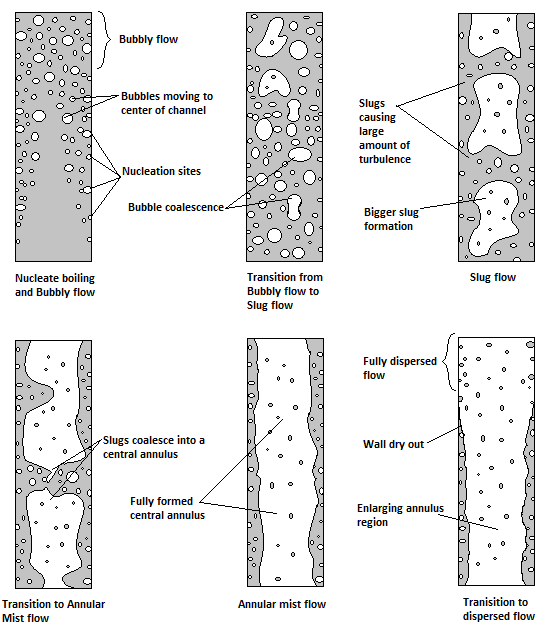
\includegraphics[width=562px]{FlowRegimePattern.png}
				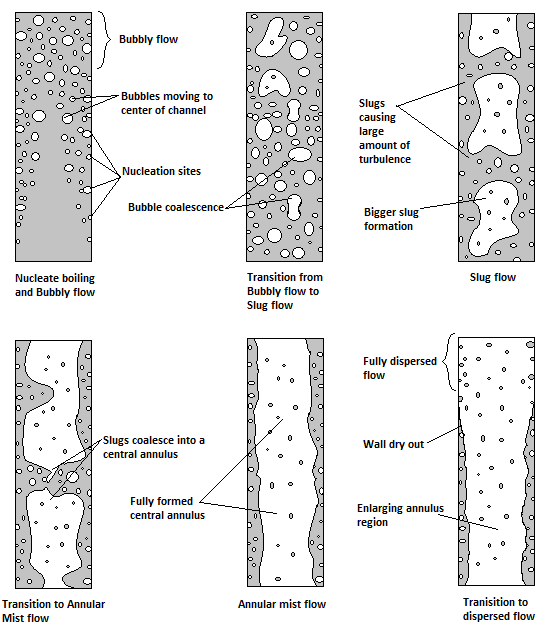
\includegraphics{FlowRegimePattern.png}
				\caption{Schematic showing different flow regimes for heat transfer below the critical heat flux (CHF).}
				\label{figure:FlowRegimePattern}
			\end{figure}
		\end{minipage}
	\end{center}
\vspace{0.5cm}
	\begin{center}
		\begin{minipage}[c]{0.85\textwidth}	
			\begin{figure}[H]
			
				%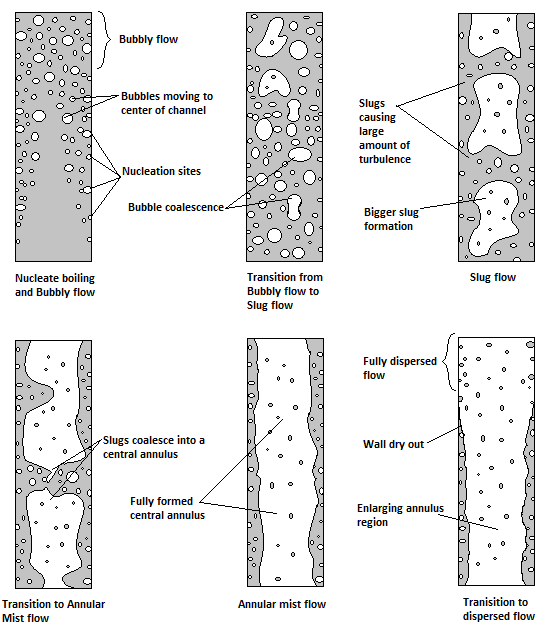
\includegraphics[width=562px]{FlowRegimePattern.png}
				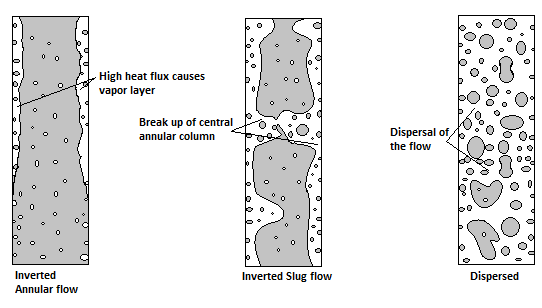
\includegraphics{CHF_FlowRegimePattern.png}
				\caption{Schematic showing different flow regimes for heat transfer above the critical heat flux (CHF).}
				\label{figure:CHF_FlowRegimePattern}
			\end{figure}
		\end{minipage}
	\end{center}
\vspace{0.5cm}


\subsection{Horizontal- versus Vertical flow}
For vertical flow the movement of bubbles is normally away from the wall (due to the liquid surface tension) symmetrically along the axis of flow because that is the direction towards which gravity is aligned. Horizontal flow has the complication that bubbles and hence the majority of the void tends to move to the upper sections of the flow channels due to buoyancy. Both these effects lead to the phenomena of \textbf{stratification}. Stratification is the process during which a multi-component fluid is segregated into its different components in such a way that the fluid no longer behaves equivalent to its fully homogenized multi-component form. Even though the study of stratification is vast, and complicated, we can use this visualization to understand that flow regimes are highly dependent on the \textbf{geometry of the flow and its orientation relative to gravity} (i.e. azimuthal angle).





\newpage
\chead{3 Test cases}
\section{Test cases}
In order to test various aspects of the thermal-hydraulic code it is necessary to construct a collection of test cases. These are:

\begin{enumerate}
\item Simple horizontal flow. No heat transfer, no junction form loss.
\item Simple horizontal flow with junction form loss.
\item Horizontal flow with heat transfer.
\item Vertical flow without heat transfer.
\item Vertical flow with heat transfer.
\end{enumerate}
\vspace{0.5cm}\noindent
For all these cases, let us use the following geometry:

	\begin{center}
		\begin{minipage}[c]{0.85\textwidth}
	
			\begin{figure}[H]
			
				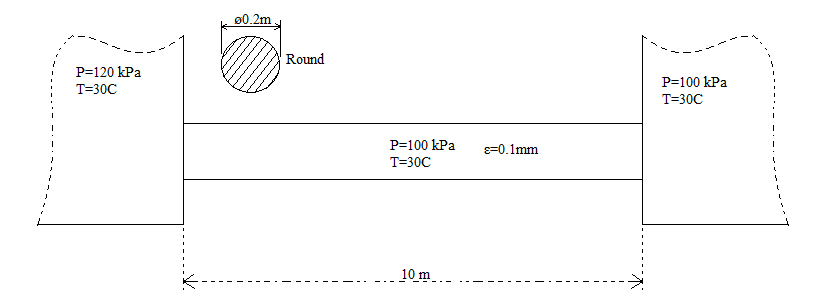
\includegraphics[width=6in]{ZZZ_TestCase.png}
				\caption{Test case geometry.}
				\label{figure:ZZZ_TestCase}
			\end{figure}
		\end{minipage}
	\end{center}
\vspace{0.5cm}













\newpage
\chead{Heat block submodel}
\section{Heat block submodel}

\subsection{The heat conduction equation}
The generalized heat conduction equation takes the following form:

\begin{equation}
\frac{dT}{dt}=\alpha \nabla^2 T + \frac{1}{\rho  C_p}\dot{e}_{gen}
\end{equation}
\newline
In slab geometry this equation takes the form:

\begin{equation}
\frac{dT}{dt}=\frac{1}{\rho  C_p} \frac{d}{dx} \biggr( k \frac{dT}{dx} \biggr) + \frac{1}{\rho  C_p}\dot{e}_{gen}
\end{equation}
\newline
And in cylindrical geometry this equation takes the form:

\begin{equation}
\frac{dT}{dt}=\frac{1}{\rho  C_p}\frac{1}{r} \frac{d}{dr} \biggr( k.r.\frac{dT}{dr} \biggr) + \frac{1}{\rho  C_p}\dot{e}_{gen}
\end{equation}
\newline
Typical boundary conditions for such second order differential equations are the symmetry or insulated boundary condition:

\begin{equation*}
\frac{dT}{dx}\biggr|_{L}=0 \quad or \quad \frac{dT}{dr}\biggr|_{R}=0
\end{equation*}
\newline
The constant temperature boundary condition:

\begin{equation*}
\frac{dT}{dt}\biggr|_{L}=0 \quad or \quad \frac{dT}{dt}\biggr|_{R}=0
\end{equation*}
\newline
And the surface convection boundary condition:

\begin{equation*}
k\frac{dT}{dx}\biggr|_L^{+,-}=h(T_L - T_{\inf})
\end{equation*}
\begin{equation*}
or
\end{equation*}
\begin{equation*}
k\frac{dT}{dr}\biggr|_R^{+,-}=h(T_R - T_{\inf})
\end{equation*}
\newline



\newpage
\subsection {Numerical form of the heat conduction equation}
Consider the nodalization as shown in Figure \ref{figure:ZZZ_HeatBlock} below.

	\begin{center}
		\begin{minipage}[c]{0.85\textwidth}
	
			\begin{figure}[H]
			
				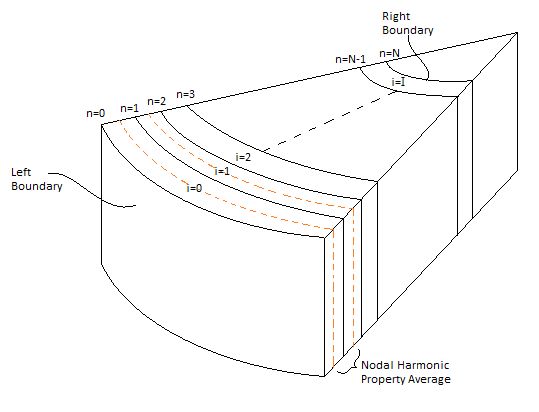
\includegraphics[width=6in]{ZZZ_HeatBlock.png}
				\caption{Heat block nodalization.}
				\label{figure:ZZZ_HeatBlock}
			\end{figure}
		\end{minipage}
	\end{center}
\vspace{0.5cm}
\noindent
\begin{comment}
We can linearize the derivatives of equation 19 as follows:

\begin{equation*}
\begin{aligned}
\frac{T_n^{t+1}-T_n^t}{\Delta t} = \frac{1}{\rho_n C_{p,n}} \frac{1}{\Delta x_n} \biggr(  k_i^t \frac{T_{n+1}^{t+1} - T_{n}^{t+1}}{\Delta x_i}  - k_{i-1}^t \frac{T_{n}^{t+1} - T_{n-1}^{t+1}}{\Delta x_{i-1}} \biggr) + \frac{1}{\rho_n C_{p,n}} \dot{e}_{gen,n}^t
\end{aligned}
\end{equation*}
\newline
Similarly, we can linearize the derivatives of equation 20 as follows:
\end{comment}
We can linearize the derivatives of equation 20 as follows:

\begin{equation}
\begin{aligned}
\frac{T_n^{t+1}-T_n^t}{\Delta t} = \frac{1}{\rho_n C_{p,n}} \frac{1}{r_n\Delta r_n} \biggr(  k_i^t.r_i. \frac{T_{n+1}^{t+1} - T_{n}^{t+1}}{\Delta r_i}  - k_{i-1}^t.r_{i-1} \frac{T_{n}^{t+1} - T_{n-1}^{t+1}}{\Delta r_{i-1}} \biggr) + \frac{1}{\rho_n C_{p,n}} \dot{e}_{gen,n}^t
\end{aligned}
\end{equation}
\newline
In this formulation the nodal points $r_1,r_2,\dots,r_N$ are defined by the user. $\Delta r_i$ is defined only on intervals. The value of $r_i$ is the halfway point between the nodes on either side of the interval. The values of $\rho_n$, $C_{p,n}$ and $\dot{e}_{gen,n}$ are calculated from the arithmetic average of the adjoining intervals as follows:
\newpage
\begin{equation*}
\begin{aligned}
\rho_n=\frac{(r_n+\half \Delta r_n)^2  -  (r_n)^2}{r_{i=n-1}^2-r_{i=n}^2} \cdot \rho_{i=n-1}
      +\frac{(r_n)^2  -  (r_n-\half \Delta r_n)^2}{r_{i=n-1}^2-r_{i=n}^2} \cdot \rho_{i=n}
\end{aligned}
\end{equation*}

\begin{equation*}
\begin{aligned}
C_{p,n}=\frac{(r_n+\half \Delta r_n)^2  -  (r_n)^2}{r_{i=n-1}^2-r_{i=n}^2} \cdot C_{p,i=n-1}
      +\frac{(r_n)^2  -  (r_n-\half \Delta r_n)^2}{r_{i=n-1}^2-r_{i=n}^2} \cdot C_{p,i=n}
\end{aligned}
\end{equation*}

\begin{equation*}
\begin{aligned}
\dot{e}_{gen,n}=\frac{(r_n+\half \Delta r_n)^2  -  (r_n)^2}{r_{i=n-1}^2-r_{i=n}^2} \cdot \dot{e}_{gen,i=n-1}
               +\frac{(r_n)^2  -  (r_n-\half \Delta r_n)^2}{r_{i=n-1}^2-r_{i=n}^2} \cdot \dot{e}_{gen,i=n}
\end{aligned}
\end{equation*}






\newpage
\subsection{Solution algorithm}
\vspace{0.5cm}\noindent
\textbf{Step 1}\newline
Load all heat block:
\begin{itemize}
\item Load mesh points, $r_n$, and initial temperatures, $T_n^t$
\item Calculate $\Delta r_n$ and $\Delta r_i$
\item Calculate intervals, $r_i$
\item Load thermal properties, $k_i$, $C_{p,i}$ and $\rho_i$
\item Load initial temperature, $T_n$
\item Set boundary conditions, $Convection$, $Symmetry$ or $Temperature$
\item Set interval heat generation, $\dot{e}_{gen,n}$
\end{itemize}

\vspace{0.5cm}\noindent
\textbf{************************* End of Initialization phase *************************}\newline

\vspace{0.5cm}\noindent
\textbf{****************** Repeat the steps below for each time step *************************}\newline


\vspace{0.5cm}\noindent
\textbf{Step 2}\newline
Set thermal conditions:
\begin{itemize}
\item Set boundary conditions, $Convection(h,T_{\inf})$, $Symmetry$ or $Temperature(T)$
\item Set interval heat generation, $\dot{e}_{gen,n}$
\end{itemize}




\vspace{0.5cm}\noindent
\textbf{Step 3a - Inner mesh points}\newline
Determine the elements of equation 21:
\begin{equation*}
\begin{aligned}
\frac{T_n^{t+1}-T_n^t}{\Delta t} = \frac{1}{\rho_n C_{p,n}} \frac{1}{r_n\Delta r_n} \biggr(  k_i^t.r_i. \frac{T_{n+1}^{t+1} - T_{n}^{t+1}}{\Delta r_i}  - k_{i-1}^t.r_{i-1} \frac{T_{n}^{t+1} - T_{n-1}^{t+1}}{\Delta r_{i-1}} \biggr) + \frac{1}{\rho_n C_{p,n}} \dot{e}_{gen,n}^t
\end{aligned}
\end{equation*}
\newline
Where the elements are:
\begin{equation*}
\begin{aligned}
B_{21}&=\frac{\Delta t}{\rho_n C_{p,n}} \cdot \frac{k_i^t.r_i        }{r_n.\Delta r_n.\Delta r_i}
 \quad and \quad
C_{21} =\frac{\Delta t}{\rho_n C_{p,n}} \cdot \frac{k_i^t.r_i        }{r_n.\Delta r_n.\Delta r_i} \\
D_{21}&=\frac{\Delta t}{\rho_n C_{p,n}} \cdot \frac{k_{i-1}^t.r_{i-1}}{r_n.\Delta r_n.\Delta r_{i-1}}
 \quad and \quad
E_{21}=\frac{\Delta t}{\rho_n C_{p,n}} \cdot \frac{k_{i-1}^t.r_{i-1}}{r_n.\Delta r_n.\Delta r_{i-1}}\\ 
F_{21}&=\frac{\Delta t}{\rho_n C_{p,n}} \dot{e}_{gen,n}^t
\end{aligned}
\end{equation*}
\newline
To get:
\begin{equation*}
\begin{aligned}
\therefore T_n^{t+1}-T_n^t&= B_{21}.T_{n+1}^{t+1} - C_{21}.T_{n}^{t+1}    
			    - D_{21}.T_{n}^{t+1} + E_{21}.T_{n-1}^{t+1}   
			    + F_{21}        
\end{aligned}
\end{equation*}
With further simplification we can write this as:

\begin{equation*}
\begin{aligned}
-E_{21}.T_{n-1}^{t+1} 
+ T_n^{t+1} + C_{21}.T_{n}^{t+1} + D_{21}.T_{n}^{t+1}
-B_{21}.T_{n+1}^{t+1}
=F_{21} + T_n^t \\
\end{aligned}
\end{equation*}
\newline
And finally:
\begin{equation}
\begin{aligned}
\biggr( -E_{21} \biggr)T_{n-1}^{t+1}
+ \biggr(1 + C_{21} + D_{21} \biggr) T_{n}^{t+1}
+ \biggr( -B_{21} \biggr)T_{n+1}^{t+1}
=\biggr( F_{21} + T_n^t \biggr) \\
\end{aligned}
\end{equation}







\vspace{0.5cm}\noindent
\textbf{Step 3b - Left convection boundary condition}\newline
This is the same as \textbf{step 3a} but with a change. For a convection boundary condition the following applies:

\begin{equation*}
k_{i-1}^t.r_{i-1} \frac{T_{n}^{t+1} - T_{n-1}^{t+1}}{\Delta r_{i-1}} \quad \to \quad h_n^t.r_n (T_{n}^{t+1}-T_{\inf,n})
\end{equation*}
\newline
Therefore, $E_{21}$ is zero and $D_{21}$ becomes:

\begin{equation*}
D_{21}=\frac{\Delta t}{\rho_n C_{p,n}} \cdot \frac{h_n^t}{\Delta r_n}
\end{equation*}
\newline 
Also $F_{21}$ now receives the known contribution from $T_{inf,n}$ and becomes:

\begin{equation*}
F_{21}=\frac{\Delta t}{\rho_n C_{p,n}} \dot{e}_{gen,n}^t + D_{21}.T_{\inf,n}
\end{equation*}




\vspace{0.5cm}\noindent
\textbf{Step 3c - Right symmetry boundary condition}\newline
This is the same as \textbf{step 3a} but with a change. For a symmetry boundary condition the following applies:

\begin{equation*}
k_i^t.r_i. \frac{T_{n+1}^{t+1} - T_{n}^{t+1}}{\Delta r_i} \quad \to \quad 0 
\end{equation*}
\newline
Therefore, $B_{21}$ and $C_{21}$ is zero with no changes to $F_{21}$.






\newpage
\vspace{0.5cm}\noindent
\textbf{Step 4}\newline
Using equation 22, in the form $\quad a_i.T_{n-1}^{t+1} + b_i.T_{n}^{t+1} + c_i.T_{n+1}^{t+1} = d_i \quad $ we can construct a linear system $Ax=b$ as follows:

\begin{equation*}
A=
\begin{bmatrix}
b_1    & c_1     & \cdots & \cdots & \cdots & 0      \\
a_2    & b_2     & c_2    & \cdots & \cdots & \vdots \\
\vdots &         & \ddots &        &        & \vdots \\
\vdots &         &        & \ddots &        & \vdots \\
\vdots &         &        &a_{I-1} &b_{I-1} &c_{I-1}  \\
0      & \cdots  & \cdots & \cdots & a_I    & b_I 
\end{bmatrix}
x=
\begin{bmatrix}
P_1^{n+1} \\
P_2^{n+1} \\
\vdots \\
\vdots \\
P_{I-1}^{n+1} \\
P_I^{n+1} 
\end{bmatrix}
b=
\begin{bmatrix}
d1 \\
d2 \\
\vdots \\
\vdots \\
d_{I-1}\\
d_I
\end{bmatrix}
\end{equation*}
\newline
This system can be solved using a conjugate gradient numerical solver.









\newpage
\chead{References}
\begin{thebibliography}{1}
	\bibitem{ChengEtAl} {\em Two-Phase Flow Patterns and Flow-Pattern Maps: Fundamentals and Applications}, ASME, Applied Mechanics Reviews, 2008.
	\bibitem{RELAP5Vol6} Shieh, A.S., Ransom, V.H., Krishnamurthy, R., {\em RELAP5/MOD3 Code Manual Volume 6: Validation of numerical techniques in RELAP5/MOD3}, NUREG/CR-5535/Rev 1.
\end{thebibliography}





\end{document}